\documentclass[12pt]{article}
\usepackage[utf8]{inputenc}
\usepackage[hyphens]{url}
\usepackage{graphicx}
\usepackage{hyperref}
\usepackage{float}
\usepackage{eurosym}
\usepackage[normalem]{ulem}
\usepackage{alltt}
\usepackage{subfig}
%\usepackage{subfigure}

% todo macro
\usepackage{color}
\newcommand{\todo}[1]{\noindent\textcolor{red}{{\bf \{ToDo}#1{\bf \}}}}

\newenvironment{code}[1]
{\begin{lrbox}{\inverbatim}\begin{minipage}{13.5cm}\begin{alltt}{#1}}
{\end{alltt}\end{minipage}\end{lrbox}\colorbox{lightgray}{\usebox{\inverbatim}}}

\newsavebox{\inverbatim}
\definecolor{lightgray}{rgb}{0.88,0.88,0.88}

\title{Semantic Web Technologies and\\ Multimedia Semantics\\ -- \\Enriching Unstructured Media Content\\ About Events to Enable Semi-Automated Summaries, Compilations, and Improved\\ Search by Leveraging Social Networks}

\date{June 2011}

\author{Thomas Steiner\\ Universitat Politècnica de Catalunya\\ Department LSI\\ 08034 Barcelona, Spain\\\\ \href{mailto:tsteiner@lsi.upc.edu}{\nolinkurl{mailto:tsteiner@lsi.upc.edu}}\\\\--\\\\Advisors:\\Joaquim Gabarr\'{o} Vall\'{e}s (UPC)\\Michael Hausenblas (DERI)\\\\--\\}
\begin{document}
\maketitle
\thispagestyle{empty}
\pagebreak 
\noindent Abstract -- Mobile devices like smartphones and digital cameras together with social networks enable people to generate, share, and consume enormous amounts of media content, both en route or at home. Common search operations, for example searching for a music clip based on artist name and song title on video platforms such as YouTube, can be achieved both based on potentially shallow human-generated metadata, or based on more profound content analysis driven by Optical Character Recognition (OCR) or Automatic Speech Recognition (ASR). However, more advanced use cases, such as summaries or compilations of several pieces of media content covering a certain event, are hard, if not impossible to fulfill at large scale. One example of such event can be a keynote speech given at a conference, where given a stable network connection media content is published on social networks while the event is still going on.

In this thesis, we develop a framework for media content processing, leveraging social networks, utilizing the Web of Data, and fine-grained media content addressing schemes like Media Fragments URIs to provide a scalable and sophisticated solution to realize the above use cases. We evaluate our approach on the entity level against social media platform APIs in conjunction with Linked (Open) Data sources, comparing the current manual approaches against our semi-automated approach. Our proposed framework can be used as an extension for existing video platforms.
\thispagestyle{empty}
\pagebreak
 
\tableofcontents
\pagebreak

\listoffigures
\listoftables
\pagebreak
 
\section{Introduction}
The lexical database WordNet~\cite{Fellbaum-WordNet-1998} by the Cognitive Science Laboratory of Princeton University defines\footnote{\url{http://wordnetweb.princeton.edu/perl/webwn?s=semantic}} the term ``semantic" as ``of or relating to meaning or the study of meaning". The same source defines\footnote{\url{http://wordnetweb.princeton.edu/perl/webwn?s=world+wide+web}} the term ``Web", which is a common form for the complete term ``World Wide Web" (or just ``WWW") as ``computer network consisting of a collection of internet sites that offer text and graphics and sound and animation resources through the hypertext transfer protocol". Finally WordNet defines\footnote{\url{http://wordnetweb.princeton.edu/perl/webwn?s=meaning}} the term ``meaning" as ``the message that is intended or expressed or signified", or ``the idea that is intended".

The combined term ``Semantic Web" has been coined by Sir Tim Berners-Lee, the inventor of the World Wide Web and Director of the World Wide Web Consortium in a May 2001 article co-published with James Hendler and Ora Lassila in the Scientific American~\cite{berners-lee_et_al_2001}. Therein, the authors write: 
\begin{quote}
``The Semantic Web will bring structure to the meaningful content of Web pages, creating an environment where software agents roaming from page to page can readily carry out sophisticated tasks for users. [\ldots]
The Semantic Web is not a separate Web but an extension of the current one, in which information is given well-defined meaning, better enabling computers and people to work in cooperation. The first steps in weaving the Semantic Web into the structure of the existing Web are already under way. In the near future, these developments will usher in significant new functionality as machines become much better able to process and ``understand" the data that they merely display at present."
\end{quote}

\subsection{The Semantic Web}
We are currently experiencing a fundamental shift from the World Wide Web (WWW) to the Semantic Web, a shift from moving bits to moving bits with a meaning. This can have a huge impact, which might not be as drastic as Tim Berners-Lee describes in his Scientific American article, but which might introduce many small improvements, like more accurate search results, or more intelligent price comparison services etc. Figure~\ref{fig:fundamental-shift} illustrates this idea.

\begin{figure}[htbp!]
\begin{center}
  \subfloat[Bits without meaning.]{\label{fig:fundamental-shift-1}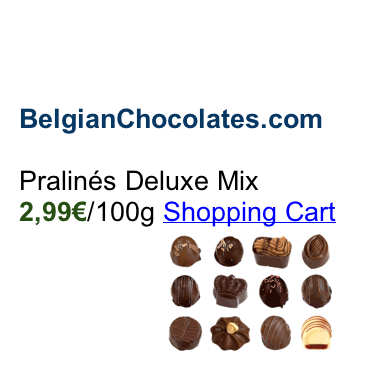
\includegraphics[width=0.3\textwidth]{./resources/fundamental-shift-1.png}}                
  \subfloat[Bits with a meaning.]{\label{fig:fundamental-shift-2}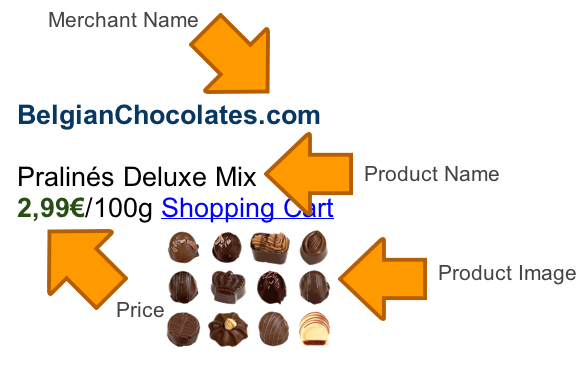
\includegraphics[width=0.468\textwidth]{./resources/fundamental-shift-2.png}}
  \caption{Fundamental shift from moving bits to moving bits with a meaning.}
  \label{fig:fundamental-shift}  
\end{center}    
\end{figure}

\subsection{The Non-Semantic Web}
To differentiate the Semantic Web from the non-semantic Web, it helps to step back one step and see why the non-semantic Web is not semantic. The Web is a system of interlinked hypertext documents accessed through the Internet. These documents are typically marked up in HTML, a language that defines a syntax understandable to user agents like Web browsers, however, not one that provides meaning beyond the level of text layout. This means that an HTML snippet like
\begin{verbatim}
<h1>The Catcher in the Rye</h1>
<h2>J. D. Salinger</h2>
\end{verbatim}
 reveals that ``The Catcher in the Rye" is a level one header element and that ``J. D. Salinger" a level two header element, but to a machine it is not evident that the prior is the title of a book, and that the latter is (i) an author, and (ii) the author of ``The Catcher in the Rye".

\subsection{Structured Data on the Web}
A very first step to add semantics to the Web is using tabular data. Table~\ref{tab:sample-table-structured-data} shows an example for such tabular data. To human beings (interested in sports), the meaning of the columns is clear:
\begin{itemize}
\item P = matches \textbf{P}layed
\item W = \textbf{W}on 
\item D = \textbf{D}rew
\item L = \textbf{L}oss
\item F = Goals \textbf{F}or
\item A = Goals \textbf{A}gainst
\item Pts = \textbf{P}oin\textbf{ts}
\end{itemize}

\begin{table}[htbp]
 \begin{center}
  \begin{tabular}{l*{6}{c}r}
Team              & P & W & D & L & F  & A & Pts \\
\hline
Manchester United & 6 & 4 & 0 & 2 & 10 & 5 & 12  \\
Celtic            & 6 & 3 & 0 & 3 &  8 & 9 &  9  \\
Benfica           & 6 & 2 & 1 & 3 &  7 & 8 &  7  \\
FC Copenhagen     & 6 & 2 & 1 & 2 &  5 & 8 &  7  \\
  \end{tabular}
\caption{Sample table with structured data for sports results.}
\label{tab:sample-table-structured-data}
 \end{center}
\end{table}

The problem, however, is for machines to understand the structure of the table. Let us imagine one wanted to automate the task of retrieving sports results. While it is a relatively straightforward job to implement a scraper bot that searches for column titles like ``P", ``W", ``D" etc., it would require the same work over and over again for different languages (for example German for: ``Sp.", ``g.", ``u.", ``v.", ``Tore", ``Pkte."). The German-speaking reader might have noticed that the exemplary German system listed here does not differentiate between ``goals for" and ``goals against", but only has a list of ``Goals". Tiny differences like this make the scraping approach so brittle. If data providers were to use unique column identifiers like URIs, the problem would be mostly gone. In the concrete example, rather than using ``D" or ``u.", which both mean that the result was a tie, the machine-readable column name could be identified by the URI \url{http://dbpedia.org/page/Tie_%28draw%29}. In the next Section we therefore introduce DBpedia.

\subsubsection{The Structured Knowledge Base DBpedia}
An often reoccurring (however not binding) pattern in the Semantic Web world is the use of DBpedia~\cite{Bizer:DBpedia} URIs as a hub for identifying concepts by URIs. DBpedia is a Semantic Web knowledge base with the objective of automatically extracting structured data from the human-generated information from the online encyclopedia Wikipedia~\cite{wikipedia}. This structured information is then made available on the World Wide Web in many variations, for example as JSON~\cite{json}, HTML~\cite{w3c_html4}, XML~\cite{Bray1998}, and many RDF~\cite{RDF} serializations. DBpedia allows for querying relationships and properties associated with Wikipedia resources, including links to other related datasets. As outlined before, the concept of a tie draw in the sense of sports could thus be uniquely identified by the DBpedia URI \url{http://dbpedia.org/page/Tie_%28draw%29}, free of all ambiguity. Similar knowledge bases are among others Freebase~\cite{NYTimes:Freebase}, YAGO~\cite{yago}, or Cyc~\cite{Cyc}.

\subsubsection{Semantics in HTML Version 4 and 5}
As outlined before, HTML versions 4~\cite{w3c_html4} and 5~\cite{w3c_html5} contain a basic level of semantics. The main focus, however, is on the separation of semantics from presentation. For example the \texttt{<b>} and the \texttt{<strong>} tags both have the same visual effect: they make the node value appear in a bold face \textbf{like so}. Visually there is no way to differentiate between the two, however, semantically the difference exists and is well-defined: \texttt{<strong>} should be used when one wants to give special emphasis on something, screenreaders will typically read out such text with a more emphasized voice. In contrast \texttt{<b>} should be used if only visually one wants to create a bold face look. In the following two Sections we present a list of semantic HTML tags and attributes and their meaning. The list is inspired by an extension\footnote{\url{https://addons.mozilla.org/en-us/firefox/addon/semantic-checker/}} for the Web browser Firefox~\cite{firefox}.

\paragraph{Semantic HTML4 Elements}
\begin{itemize}
\item \texttt{abbr} specifies an abbreviation, \texttt{acronym} specifies an acronym.
\item \texttt{h1-h6} specify level 1-6 headers, \texttt{caption} specifies a caption for a table.
\item \texttt{blockquote} specifies a block-level quotation (a source in form of a URI may be specified via the \texttt{@cite} attribute), \texttt{cite} specifies a citation.
\item \texttt{dl} specifies a definition list, \texttt{dt} specifies a definition term in a definition list, \texttt{dd} specifies the definition of a term in a definition list.
\item \texttt{em} specifies an emphasis, \texttt{strong} specifies a strong emphasis.
\item \texttt{code} specifies a code snippet, \texttt{dfn} specifies an inline definition of a single term, \texttt{address} specifies contact information for the document author, \texttt{legend} specifies a legend for \texttt{fieldset} containers for adding structure to forms, \texttt{samp} specifies sample output from a script or program.
\end{itemize}

\paragraph{Semantic HTML5 Elements}
\begin{itemize}
\item \texttt{article} specifies an independent item section of content, \texttt{aside} specifies a section of a page that consists of content that is tangentially related to the content around the \texttt{aside} element, and which could be considered separate from that content, \texttt{header} specifies a group of introductory or navigational aids, \texttt{footer} specifies a footer for its nearest ancestor sectioning content or sectioning root element, \texttt{nav} specifies a section with navigation links.
\item \texttt{figure} specifies some flow content, \texttt{mark} specifies a run of text in one document marked or highlighted for reference purposes due to its relevance in another context, \texttt{meter} specifies a scalar measurement within a known range, or a fractional value.
\item \texttt{audio} specifies a sound or an audio stream, \texttt{video} specifies a video or movie.
\item \texttt{progress} specifies the completion progress of a task, \texttt{time} specifies either a time on a 24 hour clock, or a precise date in the calendar (optionally with a time and a time-zone offset), \texttt{command} specifies a command that the user can invoke.
\item \texttt{details} specifies a disclosure widget from which the user can obtain additional information or controls, \texttt{datalist} specifies the list that represent predefined options for input elements.
\item \texttt{keygen} specifies a key pair generator control, \texttt{output} specifies the result of a calculation, \texttt{ruby} allows one or more spans of phrasing content to be marked with ruby annotations.
\end{itemize}

\paragraph{HTML5 Input Attributes}
\begin{itemize}
\item \texttt{datetime} specifies a control for setting the element's value to a string representing a global date and time (with timezone information).
\item \texttt{datetime-local} specifies a control for setting the element's value to a string representing a local date and time (with no timezone information).
\item \texttt{date} specifies a control for setting the element's value to a string representing a date, \texttt{month} specifies a control for setting the element's value to a string representing a month, \texttt{week} specifies a control for setting the element's value to a string representing a week.
\item \texttt{time} specifies a control for setting the element's value to a string representing a time (with no timezone information.
\item \texttt{number} specifies a control for setting the element's value to a string representing a number.
\item \texttt{range}  represents an imprecise control for setting the element's value to a string representing a number.
\item \texttt{email} specifies a control for editing a list of email addresses given in the element's value.
\item \texttt{url} specifies a control for editing an absolute URL given in the element's value.
\item \texttt{search} specifies a one-line plain-text edit control for entering one or more search terms.
\item \texttt{color} specifies a color-well control for setting the element's value to a string representing a simple color.
\end{itemize}

\subsection{Structured Data Beyond Pure HTML}
In this Section we describe how structured data can be included in HTML documents by either overloading existing HTML attributes, or by adding new HTML attributes.

\subsubsection{Microformats}
Microformats~\cite{microformats} are a set of open data mark-up formats developed and defined by the Microformats community\footnote{\url{http://microformats.org/discuss}}. Microformats are not an official standard, but rather a widely adopted grass-roots-driven movement with origins in the blogging scene. It is to be noted that Microformats do not require a new language, but reuse building blocks from widely adopted standards such as the \texttt{@class}, \texttt{@rel}, and \texttt{@title} attributes in HTML. Its main design goal is to focus first on humans, then on machines. A concrete example of Microformat mark-up in HTML can be seen in Figure~\ref{code:microformats}. There are currently nine stable Microformats\footnote{\url{http://microformats.org/wiki/Main_Page\#Specifications}}, as listed below:
\begin{itemize}
\item \texttt{hCalendar} is a distributed calendaring and events format, using a 1:1 representation of the standard \texttt{iCalendar} format (RFC2445,~\cite{Dawson:1998:ICS:RFC2445}).
\item \texttt{hCard} is a format for representing people, companies, organizations, and places, using a 1:1 representation of the standard \texttt{vCard} format (RFC2426,~\cite{Dawson:1998:VMD:RFC2426}).
\item \texttt{rel-license} is a format for indicating content licenses, which is embeddable in HTML~\cite{w3c_html4} or XHTML~\cite{xhtml10sec}, Atom~\cite{Atom:Synd}, RSS~\cite{rss2006rss}, and arbitrary XML~\cite{Bray1998}.
\item \texttt{rel-nofollow} is a format for hyperlinks indicating that the destination of that hyperlink should not be afforded any additional weight or ranking by user agents such as search engines, which perform link analysis upon Web pages.
\item \texttt{rel-tag} format for hyperlinks indicating that the destination of that hyperlink is an author-designated keyword for the current page.
\item \texttt{VoteLinks} is a format for adding the idea of agreement, abstention or indifference, and disagreement to hyperlinks.
\item \texttt{XFN} is a format for representing human relationships using hyperlinks, which enables Web authors to indicate their relationships to people.
\item \texttt{XMDP} is a format for defining metadata profile documents (XHTML Meta Data Profile), which enables Web authors to well-define custom meta tags.
\item \texttt{XOXO} is a format for defining a new XHTML document type for subsetting and extending XHTML, which serves as the basis for XHTML-friendly outlines for processing by XML engines, and for easy interactive rendering by browsers.
\end{itemize}

\begin{figure}[htbp!]
\begin{center}
{\footnotesize
\begin{code}
<div class="\uwave{vcard}">
  <a class="\uwave{fn org url}" href="http://www.commerce.net/">CommerceNet</a>
  <div class="\uwave{adr}">
    <span class="\uwave{type}">Work</span>:
    <div class="\uwave{street-address}">169 University Avenue</div>
    <span class="\uwave{locality}">Palo Alto</span>,  
    <abbr class="\uwave{region}" title="California">CA</abbr>&nbsp;&nbsp;
    <span class="\uwave{postal-code}">94301</span>
    <div class="\uwave{country-name}">USA</div>
  </div>
  <div class="\uwave{tel}">
   <span class="\uwave{type}">Work</span> +1-650-289-4040
  </div>
  <div class="\uwave{tel}">
    <span class="\uwave{type}">Fax</span> +1-650-289-4041
  </div>
  <div>Email: 
   <span class="\uwave{email}">info@commerce.net</span>
  </div>
</div>
\end{code}}
  \caption[Sample code snippet with embedded hCard Microformat mark-up.]{Sample code snippet with embedded \texttt{hCard} \uwave{Microformat} mark-up. Source: \url{http://microformats.org/wiki/hcard}}
  \label{code:microformats} 
  \end{center}  
\end{figure}

\subsubsection{RDFa}
RDFa~\citation{ben_adida_rdfa_2008} stands for RDF in attributes, and is a specification for the expression of structured data in any mark-up language like for example XHTML~\cite{xhtml10sec}. RDF is explained in more detail in Section~\ref{sec:rdf}, its main idea is to express statements about things in the form of subject, predicate, object triples. RDFa shares some design goals with Microformats~\cite{microformats}. Where Microformats specify both a syntax for embedding structured data into HTML \emph{and} a vocabulary of specific terms for each Microformat, RDFa in contrast \emph{only} specifies a syntax. RDFa relies on independent external specifications of vocabularies. The essence of RDFa is a set of attributes that contain metadata about things, and that can be embedded in mark-up languages, for example in XHTML or HTML. The concrete attributes are:
\begin{itemize}
\item \texttt{about} and \texttt{src}: a URI or CURIE (compact URI expressions) specifying the resource the metadata is about.
\item \texttt{rel} and \texttt{rev}: specifying a relationship or reverse-relationship with another resource.
\item \texttt{href} and \texttt{resource}: specifying the partner resource.
\item \texttt{property}: specifying a property for the content of an element.
\item \texttt{content}: optional attribute that overrides the content of the element when using the property attribute.
\item \texttt{datatype}: optional attribute that specifies the datatype of text specified for use with the property attribute.
\item \texttt{typeof}: optional attribute that specifies the RDF type(s) of the subject (the resource that the metadata is about).
\end{itemize}
An example of RDFa in HTML can be seen in Figure~\ref{code:rdfa}.

\begin{figure}[htbp!]
\begin{center}
{\footnotesize
\begin{code}
<html
  xmlns="http://www.w3.org/1999/xhtml"
  \uwave{prefix}="foaf: http://xmlns.com/foaf/0.1/
          dcterms: http://purl.org/dc/terms/"
>
  <head>
    <title>My home-page</title>
    <meta \uwave{property}="dcterms:creator" \uwave{content}="Mark Birbeck" />
    <link \uwave{rel}="foaf:topic" \uwave{href}="http://www.example.com/#us" />
  </head>
  <body>...</body>
</html>
\end{code}}
  \caption[Sample code snippet with RDFa mark-up.]{Sample code snippet with \uwave{RDFa} mark-up. Source: \url{http://www.w3.org/TR/rdfa-core/}}
  \label{code:rdfa} 
  \end{center}  
\end{figure}

\subsubsection{Microdata}
Microdata~\cite{Hickson:Microdata10} defines a way to annotate content (or items) with specific machine-readable labels, for example to allow scripts to provide services that are customized to a website. Microdata allows nested groups of name-value pairs to be added to documents, in parallel with the existing content. The Microdata specification introduces a set of new attributes to HTML:
\begin{itemize}
\item \texttt{itemscope}: creates an item (or thing) and indicates that descendants of this element contain information about it. This attribute precedes the \texttt{itemtype} attribute in the HTML element’s tag.
\item \texttt{itemtype}: a valid URL of a vocabulary that describes the item and its properties context.
\item \texttt{itemid}: indicates a unique identifier of the item in the vocabulary.
\item \texttt{itemprop}: indicates that its containing tag holds the value of the specified item property. The properties name and value context are described by the items vocabulary. Properties values usually consist of string values, but can also use URLs using the \texttt{a} element and its \texttt{href} attribute, the \texttt{img} element and its \texttt{src} attribute, or other elements that link to or embed external resources.
\item \texttt{itemref}: properties that are not descendants of the element with the \texttt{itemscope} attribute can be associated with the item using this attribute. Provides a list of elements to web crawlers to find additional property values of the item elsewhere in the document.
\end{itemize}

An example of Microdata in HTML can be seen in Figure~\ref{code:microdata}

\begin{figure}[htbp!]
\begin{center}
{\footnotesize
\begin{code}
<div \uwave{itemscope}>
  <p>My name is <span \uwave{itemprop}="name">Neil</span>.</p>
  <p>
    My band is called
    <span \uwave{itemprop}="band">Four Parts Water</span>.
  </p>
  <p>I am <span \uwave{itemprop}="nationality">British</span>.</p>
</div>
\end{code}}
  \caption[Sample code snippet with \uwave{Microdata} mark-up.]{Sample code snippet with Microdata mark-up. Source: \url{http://www.w3.org/TR/microdata/}}
  \label{code:microdata} 
\end{center}    
\end{figure}

\subsection{Linked Data}
Linked Data~\cite{TimBL:LinkedData} defines a set of agreed-on best practices and principles for interconnecting and publishing structured data on the Web. It uses Web technologies like HTTP~\cite{fielding1999hypertext} and URIs~\cite{bernerslee2005uri} to create typed links between different sources. The portal LinkedData.org defines Linked Data as being ``about using the Web to connect related data that wasn't previously linked, or using the Web to lower the barriers to linking data currently linked using other methods". 

\subsubsection{The Linked Data Principles}
Tim Berners-Lee defines the four rules for Linked Data in a W3C Design Issue~\cite{TimBL:LinkedData} as follows:
\begin{enumerate}
\item Use URIs as names for things.
\item Use HTTP URIs so that people can look up those names.
\item When someone looks up a URI, provide useful information, using the standards (RDF*, SPARQL).
\item Include links to other URIs, so that they can discover more things.
\end{enumerate}

Linked Data uses RDF~\cite{RDF} to create typed links between things in the world, the result is oftentimes referred to as the Web of Data. As outlined before, RDF encodes statements about things in the form of subject, predicate, object triples. If subject and object have URIs from different namespaces, Bizer et al. speak of ``RDF links" in~\cite{bizer07how}. An examplary RDF link taken from~\cite{BizerHB09} stating that a description of the movie Pulp Fiction from the Linked Movie Database~\cite{HasCon09} and from DBpedia are in fact talking about the same movie can be seen in Figure~\ref{code:rdflink}.

\begin{figure}[htbp!]
\begin{center}
{\footnotesize
\begin{code}
http://data.linkedmdb.org/resource/film/77
http://www.w3.org/2002/07/owl\#sameAs
http://dbpedia.org/resource/Pulp\_Fiction\_\%28film\%29
\end{code}}
  \caption[Exemplary RDF link.]{Exemplary RDF link stating that a description of the movie Pulp Fiction from the Linked Movie Database~\cite{HasCon09} and from DBpedia are in fact talking about the same movie.}
  \label{code:rdflink} 
\end{center}    
\end{figure}

\subsubsection{The Linked Open Data Cloud}\label{sec:lodcloud}
The Linking Open Data (LOD) project~\cite{lodproject} is the most visible Linked Data effort. The project's objective is to indentify existing datasets with open licenses, convert them to RDF whilst obeying the Linked Data principles, and finally publish them on the Web. Due to its open structure everyone can contribute to the project by publishing a dataset and interlinking it to existing datasets. Today, the project includes datasets of big names such as the BBC, Thomson Reuters, or the Library of Congress to name just a few. The current state of the Linking Open Data project can be seen in the so-called Linked Open Data cloud, a diagram that depicts the interconnectedness of each dataset. The state of the LOD cloud as of September 2010 can be seen in Figure~\ref{fig:lod-cloud}.
\begin{figure}[htbp!]
\begin{center}
    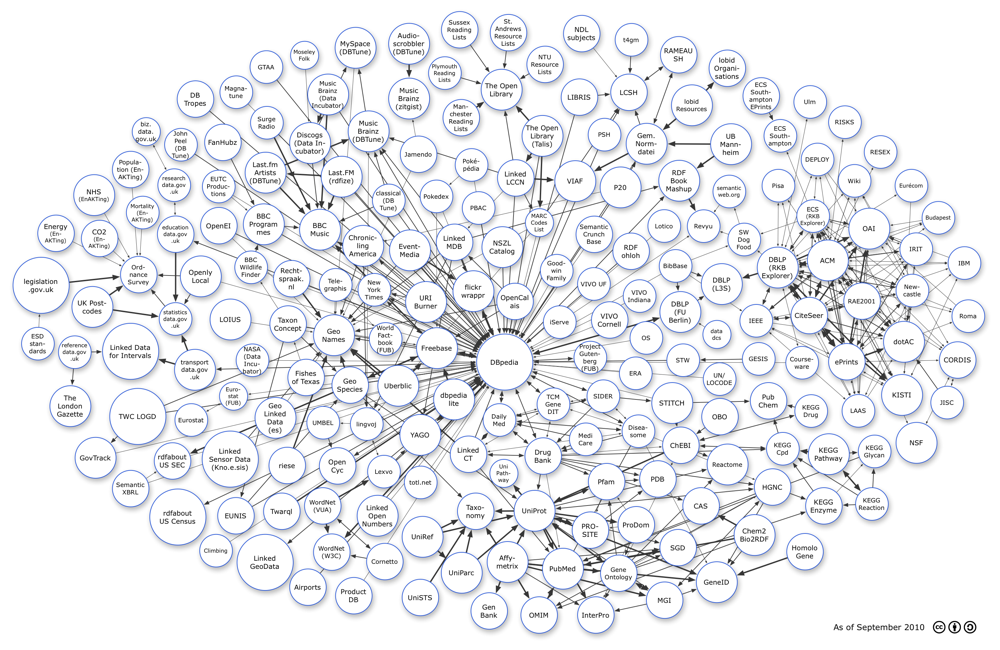
\includegraphics[width=1.0\textwidth]{./resources/lod-cloud.png}    
  \caption[The Linked Open Data cloud as of September 2010.]{The Linked Open Data cloud as of September 2010, by Richard Cyganiak and Anja Jentzsch. Source: \url{http://lod-cloud.net/}}    
  \label{fig:lod-cloud}
  \end{center}  
\end{figure}

\section{State of the Art in Multimedia Semantics}
The term ``multimedia" is defined\footnote{\url{http://wordnetweb.princeton.edu/perl/webwn?s=multimedia}} by WordNet as ``transmission that combine media of communication (text and graphics and sound etc.)". We use the term in the context of the Web, that is, in the sense of video on the Internet. While other technologies (such as interactive Adobe Flash\footnote{\url{http://get.adobe.com/flashplayer/}} applications) also fulfill the definition, we focus ourselves on open, plug-in free technologies, based on the HTML5~\cite{w3c_html5} Working Draft. Given the previously introduced definition of ``semantics" (``of or relating to meaning or the study of meaning"), we can then define the combined term ``multimedia semantics" as the process of giving meaning to video files on the Web. Official statistics~\cite{youtube:stats} from YouTube~\cite{youtube}, one of the biggest online video platforms, say that more than 13 million hours of video were uploaded during 2010, and 35 hours of video are uploaded every minute.

\subsection{The Semantic Gap}
Mostly text-based video search engines such as YouTube~\cite{youtube}, Bing Videos~\cite{bing}, Yahoo! Videos~\cite{yahoo}, or Google Videos~\cite{google} work mainly based on filenames, textual descriptions, video titles, or user tags, but do not take semantics into account: they do not get the meaning of a video, for example whether a video tagged with ``obama" is about \textit{the} Obama, or about a person that just happens to have the same name. In addition to that videos have a temporal dimension that with today's adaptive video codecs like VP8~\cite{vp8} does not directly map back to discrete units within the video like frames. In~\cite{Smeulders}, Smeulders et al. define the semantic gap as
\begin{quotation}
\noindent ``The semantic gap is the lack of coincidence between the information that one can extract from the visual data and the interpretation that the same data have for a user in a given situation."
\end{quotation}

\noindent The semantic gap is visualized in Figure~\ref{fig:semantic-gap}. While the shapes and colors can be easily extracted, the overall meaning is hard to understand for machines. This is especially true for moving images as in video content.

\begin{figure}[htbp!]
\begin{center}
 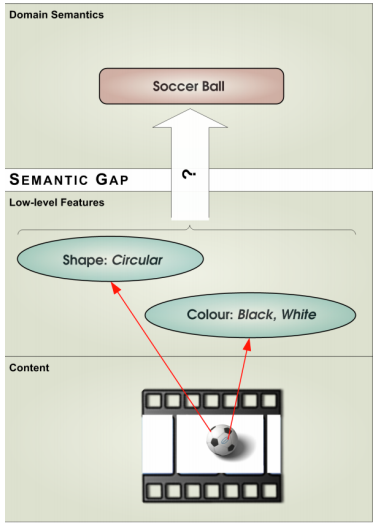
\includegraphics[width=0.4\linewidth]{./resources/semantic-gap.png}
 \caption[The semantic gap visualized.]{The semantic gap visualized. Source:~\cite{Hausenblas:PhD08}}
  \label{fig:semantic-gap}
  \end{center}  
\end{figure}

In the following we describe two approaches to bridge the semantic gap. One well-known and established, and one new and not yet broadly known.

\subsection{MPEG-7}
The formal name of MPEG-7~\cite{mpeg7} is Multimedia Content Description Interface. Unlike MPEG-1, -2, and -4, MPEG-7 does not deal with the actual encoding of moving pictures and audio, but rather stores metadata in XML format in order to describe multimedia content. MPEG-7 is meant to complement the previous MPEG standards, however, can also be used on its own independently. Quoting from MPEG-7: The Generic Multimedia Content Description Standard, Part 1~\cite{mpeg7}:
\begin{quotation}
\noindent ``A Description consists of a Description Scheme (structure) and the set of Descriptor Values (instantiations) that describe the Data."
\end{quotation}

\subsubsection{Components of MPEG-7}
While one requirement of MPEG-7 is that the description must be separate from the audiovisual content, there must be a relation between the content and the description, which is why it is multiplexed with the content itself. Essentially MPEG-7 consists of three components:
\begin{description}
\item [Descriptors:] Are used to describe the specific features of a multimedia file. Such features can be the color or the title of a scene, but also the semantic description of it. 
\item [Description Schemes:] Are pre-defined descriptor structures that are put in relation to each other. Such relations can be between descriptors and descriptor schemes, or between descriptor schemes among each other.
\item [Description Definition Language (DDL):] Is a language for defining and extending descriptors and descriptor schemes. DDL is an extension of XML Schema~\cite{xmlschema1sec},~\cite{xmlschema2sec}.
\end{description}

\subsubsection{Issues of MPEG-7}
In a critical view of MPEG-7, Hausenblas et al. point out in~\cite{Hau07}:

\begin{quotation}
\noindent ``Due to the wide application, the semantics of the description tools are often very general. Several works have already pointed out the lack of formal semantics of the standard that could extend the traditional text descriptions into machine understandable ones. [\ldots] Profiles [\ldots] have been proposed as a means to reduce the complexity of MPEG-7 descriptions. Like in other MPEG standards, profiles are subsets of the standard that cover certain functionalities [\ldots]. In MPEG-7, profiles are subsets of description tools for certain application areas [\ldots]."
\end{quotation}

\noindent In~\cite{Celma2007}, Celma et al. detail the problem with metadata interoperability in MPEG-7, mainly due to the lack of precise semantics. The authors explain that semantically identical metadata can be represented in multiple ways. For example an image depicting a player scoring a goal can be annotated using the free text tag, or using the keyword tag. The term ``ontology" in the context of computer science is according to WordNet defined\footnote{\url{http://wordnetweb.princeton.edu/perl/webwn?s=ontology}} as ``a rigorous and exhaustive organization of some knowledge domain that is usually hierarchical and contains all the relevant entities and their relations". Efforts have been made to translate MPEG-7 into an ontology and through appropriate frameworks to enable its integration with other ontologies, thus enhancing interoperability, however, these efforts did not gain the traction their authors had hoped for.

\subsection{Ontology for Media Resources}
The W3C Ontology for Media Resources~\cite{mediaontology} defines a set of mappings~\cite{mappingtable} for many existing metadata formats. This ontology aims to foster the interoperability among various kinds of metadata formats currently used to describe media resources on the Web. Using the Ontology for Media Resources, time based semantic annotations are possible using the \texttt{relation} property to link to an RDF file or named graph containing annotations for a media resource (or fragment). Currently there is no solution for embedding a set of RDF triples directly into one of the properties of the Ontology for Media Resources.

\section{Resource Description Framework (RDF)}\label{sec:rdf}
The Resource Description Framework (RDF)~\cite{RDF} defines a set of W3C standards for the formal description of resources that are identified by URIs. RDF is a core component of the Semantic Web. Initially it was designed to describe metadata on the World Wide Web (WWW) such as authors, copyrights, etc. of documents, however, using a definition of the term ``resource" beyond the WWW context, RDF is now also used to describe metadata of any URI-identifiable entity.

\subsection{Triples as a Data Structure}
As outlined before, one of the main purposes of the Semantic Web is to give information a well-defined meaning. Using an example from Berners-Lee's article~\cite{berners-lee_et_al_2001}, meaning can be to differentiate between the concepts of a shipping and a billing address, or the concept of an address in the sense of delivering a formal spoken communication to an audience. In order to assure the differences in meaning, things are identified by a Unique Resource Identifier (URI). The majority of the data processed by machines can be described by elementary sentences like ``A cat is a mammal", ``Thomas Steiner is author of this document", or ``Prince William is married to Kate Middleton". Each of these sentences has a subject (``A cat"), a predicate (``is a "), and an object (``mammal"). Every subject, predicate, and object can be identified by a URI. This concept turns out to be very powerful, as it allows to express the same concept, represented by a URI (like for example mammal by \url{http://dbpedia.org/resource/Mammal}) with different terms in different languages (like for example Säugetier, mammal, or nisäkkäät). Everyone can extend the set of concepts, simply by creating a URI on the Web. This form of knowledge representation is used by the Resource Description Framework, or short RDF~\cite{RDF}.

\subsection{Important RDF Serialization Syntaxes}
The knowledge represented in the RDF triple data structure needs to be serialized in order to be stored or transmitted over the Internet. Several serialization formats exist, each of which has its particular advantages and disadvantages, mostly around readability for human beings and parseability for machines. Most people prefer the Turtle~\cite{turtle} format for its readability, whereas for machines N-Triples~\cite{rdf-n-triples} is the easiest to parse.

\subsubsection{RDF Sample Graph}
In the following we will illustrate the various RDF serialization formats with an RDF sample graph, which is introduced here. It contains data about a FOAF~\cite{FOAF} person that has the name ``John X. Foobar", and an email address with an SHA1~\cite{sha1} checksum of `cef817456278b70cee8e5a1611539\-ef9d928810e". The email is obscured for spam reasons. Figure~\ref{fig:sample-rdf-graph} shows the graphical representation of this sample graph.

\begin{figure}[htbp!]
\begin{center}
 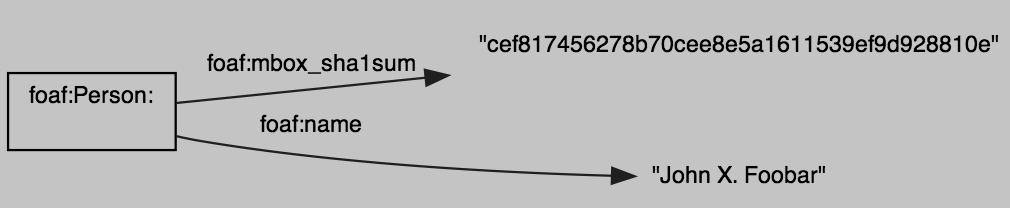
\includegraphics[width=\linewidth]{./resources/sample-rdf-graph.png} 
 \caption{A sample RDF graph visualized.}
 \label{fig:sample-rdf-graph}
 \end{center}  
\end{figure}

\subsubsection{The Notation3 Syntax} \label{sec:notation3}
Notation3 (sic)~\cite{BernersLee2008} was introduced by Tim Berners-Lee. Notation3 has some features that go beyond the pure expressiveness of RDF, like rules. Its media type is \texttt{text/n3;\-charset=utf-8}, the recommended file extension is \texttt{.n3}, the encoding is always UTF-8. Figure~\ref{code:notation3-syntax} shows the previously introduced sample graph serialized in Notation3.
\begin{figure}[htbp!]
\begin{center}
{\footnotesize
\begin{code}
@prefix foaf: <http://xmlns.com/foaf/0.1/> .

_:node15urahancx74223 a foaf:Person ;
  foaf:name "John X. Foobar" ;
  foaf:mbox_sha1sum "cef817456278b70cee8e5a1611539ef9d928810e" .
\end{code}}
  \caption{A sample graph in Notation3 syntax.}
  \label{code:notation3-syntax}
  \end{center}  
\end{figure}

\subsubsection{The Turtle Syntax} \label{sec:turtle}
Turtle~\cite{turtle} was developed by Dave Beckett and Tim Berners-Lee. It is a superset of N-Triples (see Section~\ref{sec:n-triples}) and a subset of Notation3 (see Section~\ref{sec:notation3}). While at the time of writing it is not yet an officially recognized standard, it has reached a de facto standard status. Its media type is \texttt{text/turtle} (the sometimes still observable media type \texttt{application/x-turtle} is deprecated), the recommended file extension is \texttt{.ttl}, the encoding is UTF-8. Figure~\ref{code:turtle-syntax} shows the previously introduced sample graph serialized in Turtle.

\begin{figure}[htbp!]
\begin{center}
{\footnotesize
\begin{code}
@prefix foaf: <http://xmlns.com/foaf/0.1/> .

_:node15urahancx74223 a foaf:Person ;
  foaf:name "John X. Foobar" ;
  foaf:mbox_sha1sum "cef817456278b70cee8e5a1611539ef9d928810e" .
\end{code}}
  \caption{A sample graph in Turtle syntax.}
  \label{code:turtle-syntax}
  \end{center}  
\end{figure}

\subsubsection{The N-Triples Syntax} \label{sec:n-triples}
The N-Triples~\cite{rdf-n-triples} syntax was developed by the W3C RDF-Core Working Group. N-Triples is a subset of Turtle (see Section~\ref{sec:turtle}), which in turn is a subset of Notation3 (see Section~\ref{sec:notation3}). There are very few variations to express a graph in N-Triples, which makes it an ideal syntax for testing purposes, however, as it is missing some shortcuts of Turtle, it is quite verbose. Its media type is \texttt{text/plain}, the recommended file extension is \texttt{.nt}, and the encoding is 7-bit US-ASCII. Figure~\ref{code:ntriples-syntax} shows the previously introduced sample graph serialized in N-Triples.

\begin{figure}[htbp!]
\begin{center}
{\footnotesize
\begin{code}
\_:1 <http://www.w3.org/1999/02/22-rdf-syntax-ns#type>
    <http://xmlns.com/foaf/0.1/Person> .
\_:1 <http://xmlns.com/foaf/0.1/name>
    "John X. Foobar" .
\_:1 <http://xmlns.com/foaf/0.1/mbox_sha1sum>
    "cef817456278b70cee8e5a1611539ef9d928810e" .
\end{code}}
  \caption{A sample graph in N-Triples syntax.}
  \label{code:ntriples-syntax}
  \end{center}  
\end{figure}

\subsubsection{The RDF/XML Syntax}
RDF/XML~\cite{Beckett2004} was introduced by the W3C as the first RDF serialization syntax. It is still the only officially recommended standard, albeit more human-friendly serialization formats such as Turtle are gaining more and more traction. Its media type is \texttt{application/rdf+xml}, the recommended file extension is \texttt{.rdf}, the encoding is UTF-8. Figure~\ref{code:rdfxml-syntax} shows the previously introduced sample graph serialized in RDF/XML.

\begin{figure}[htbp!]
\begin{center}
{\footnotesize
\begin{code}
<?xml version="1.0" encoding="UTF-8"?>
<rdf:RDF
    xmlns:foaf="http://xmlns.com/foaf/0.1/"
    xmlns:rdf="http://www.w3.org/1999/02/22-rdf-syntax-ns#">
  <rdf:Description rdf:nodeID="node15urahancx74224">
    <rdf:type rdf:resource="http://xmlns.com/foaf/0.1/Person"/>
    <foaf:name>John X. Foobar</foaf:name>
    <foaf:mbox_sha1sum>
      cef817456278b70cee8e5a1611539ef9d928810e
    </foaf:mbox_sha1sum>
  </rdf:Description>
</rdf:RDF>
\end{code}}
  \caption{A sample graph in RDF/XML syntax.}
  \label{code:rdfxml-syntax}
  \end{center}  
\end{figure}

\subsubsection{The RDFa Syntax}
RDFa has a special role in that it is a specification for attributes to express structured data in XHTML~\cite{ben_adida_rdfa_2008} (but also standard HTML). It uses the rendered hypertext content of XHTML for the RDFa markup, so that data publishers can use the same document for human- and machine-readable content. There is also a specification for RDFa 1.1 in HTML4 and HTML5~\cite{rdfa:html}. The contained RDF triples can be extracted with distillers, in consequence RDFa can be considered as another serialization syntax for RDF, with the same expressive power as RDF/XML or Turtle. Its media type is \texttt{application/xhtml+xml}, the recommended file extension is \texttt{.html}. Figure~\ref{code:rdfa-syntax} shows the previously introduced sample graph serialized in RDFa.

\begin{figure}[htbp!]
\begin{center}
{\footnotesize
\begin{code}
<div about="_:1" typeof="http://xmlns.com/foaf/0.1/Person">           
  <span property="http://xmlns.com/foaf/0.1/mbox_sha1sum">
    cef817456278b70cee8e5a1611539ef9d928810e
  </span> 
  <span property="http://xmlns.com/foaf/0.1/name">
    John X. Foobar
  </span>
</div> 
\end{code}}
  \caption{A sample graph in RDFa syntax.}
  \label{code:rdfa-syntax}
  \end{center}  
\end{figure}

\subsection{RDFa with the Example of Annotating a Photo Website}
In this Section we give a quick overview on how image websites can use RDF in the form of RDFa to publish license data about their images. Given a well-defined license, image search services like Bing image search~\cite{bingimg} or Google image search~\cite{googleimg} can use this license information for facilitating users the process of finding openly licensed or commercially modifiable images. Search engines oftentimes allow for specifying a desired license in their advanced search features~\cite{googleadvancedimg}.

\begin{figure}[htbp!]
\begin{center}
{\footnotesize
\begin{code}
<!-- First image -->
<img \uwave{src}="http://imgs.xkcd.com/comics/debian_main.png"
     title="dpkg: error processing package (--purge):
         subprocess pre-removal script returned error exit 163:
         OH_GOD_THEYRE_INSIDE_MY_CLOTHES" 
     alt="debian-main"
/>
This work is licensed under a
<a \uwave{about}="http://imgs.xkcd.com/comics/debian_main.png"
   \uwave{rel}="license" 
   \uwave{href}="http://creativecommons.org/licenses/by-nc/2.5/">
  Creative Commons Attribution-NonCommercial 2.5 License
</a>.

<!-- Second image -->
<img \uwave{src}="http://imgs.xkcd.com/comics/marie_curie.png"
     title="Although not permanently."
     alt="Marie Curie"
/>
<a \uwave{about}="http://imgs.xkcd.com/comics/marie_curie.png"
   \uwave{rel}="license"
   \uwave{href}="http://creativecommons.org/licenses/by-nc/2.5/">
  Creative Commons Attribution-NonCommercial 2.5 License
</a>.
\end{code}}
  \caption[License information about a set of images expressed in RDFa.]{License information about a set of images expressed in \uwave{RDFa}. The \texttt{about} attribute in the anchor tags binds the license to the particular image resources identified by the images' URLs in the \texttt{src} attribute of the image tags.}
  \label{code:rdfa-license}
  \end{center}  
\end{figure}

\section{SPARQL - Semantic Web Query Language}
SPARQL is a recursive acronym that stands for SPARQL Protocol and RDF Query Language. The SPARQL specification~\cite{sparql} defines the syntax and semantics of the SPARQL query language for RDF. RDF~\cite{RDF} is a directed, labeled graph data format for representing information in the Web. SPARQL can be used to express queries across diverse data sources, whether the data is stored natively as RDF, or viewed as RDF via middleware. SPARQL allows for querying required and optional graph patterns along with their conjunctions and disjunctions. SPARQL also supports extensible value testing and constraining queries by source RDF graph. The results of SPARQL queries can be results sets or RDF graphs.

SPARQL became an official World Wide Web Consortium (W3C) Recommendation in the year 2008. It was standardized by the RDF Data Access Working Group (DAWG).

\subsection{The Vision of the Web as a Giant, Single Database}
The Web as we know it today is a \emph{network of documents} interconnected by hyperlinks that everyone can participate in by placing links to existing documents. The vision of the Semantic Web, however, is a \emph{network of facts} about entities, interconnected in form of graphs of data. Where the Web of today is a graph of documents, the Semantic Web is envisioned to be a huge global graph, formed by many, many individual graphs. If one party publishes facts about an entity, and a different party publishes different facts about the same entity, then the overall knowledge about that entity is represented in a decentralized way, accessible to all, and open for everyone to enrich. This obviously requires strong globally unique identifiers, or at least ways to map one identifier to another.

Given the (visionary) huge global graph, a SPARQL query like the one in Figure~\ref{code:sparql} could be used to get results from the graph, like the email addresses of every person in the world.

\begin{figure}[htbp!]
\begin{center}
{\footnotesize
\begin{code}
PREFIX foaf: <http://xmlns.com/foaf/0.1/>
SELECT ?name ?email
WHERE {
  ?person a foaf:Person.
  ?person foaf:name ?name.
  ?person foaf:mbox ?email.
}
\end{code}}
  \caption[SPARQL query returning the names and email addresses of every person in the world.]{SPARQL query returning the names and email addresses of every person in the world. Source: \url{http://en.wikipedia.org/wiki/SPARQL\#Benefits}} 
  \label{code:sparql}
  \end{center}  
\end{figure}

This query selects the names and email addresses from all persons who have facts about them in the global graph. The query starts with a prefix definition, and then constrains the results to be of type \texttt{foaf:Person}, whose name and email address are the values of the triples with the predicates \texttt{foaf:name} and \texttt{foaf:mbox} respectively. While this sounds like a very powerful idea, for performance reasons in practice SPARQL endpoints like the DBpedia SPARQL endpoint~\cite{dbpedia:sparql} typically only allow for querying the local graph.

\subsection{Different SPARQL Query Variations}
The SPARQL Query Language currently specifies four different query variants, which we list in the following. 

\subsubsection{SELECT}
The \texttt{SELECT} query variant is used to extract raw values from a SPARQL endpoint. The results are returned in a table format. A sample query is given in Figure~\ref{code:sparql}.

\subsubsection{DESCRIBE}
The \texttt{DESCRIBE} query variant is used to extract an RDF graph from the SPARQL endpoint, the contents of which is left to the endpoint to decide based on what the maintainer deems as useful information. An example query is given below:\\

\texttt{DESCRIBE <http://example.org/sparql>}

\subsubsection{ASK}
The \texttt{ASK} query variant is used to provide a simple True/False result for a query on a SPARQL endpoint. No information is returned about the possible query solutions, just whether or not a solution exists. An example query with a sample response is given below:\\

\noindent Given the following SPARQL \texttt{ASK} query:\\

\texttt{PREFIX foaf: <http://xmlns.com/foaf/0.1/>\\
\indent ASK \{ ?x foaf:name  "Alice" \}}\\

\noindent Creates the following response (given there is a person named Alice):\\

\texttt{yes}

\subsubsection{CONSTRUCT}
The \texttt{CONSTRUCT} query variant is used to extract information from the SPARQL endpoint and transform the results into valid RDF specified by a graph template. The result is an RDF graph formed by taking each query solution in the solution sequence, substituting for the variables in the graph template, and combining the triples into a single RDF graph by set union. An example query is given below:\\

\noindent Given the following RDF graph:\\

\texttt{@prefix foaf: <http://xmlns.com/foaf/0.1/> .}\\
\texttt{\indent \_:a foaf:name "Alice" .}\\
\texttt{\indent \_:a foaf:mbox <mailto:alice@example.org> .}\\

\noindent And given the following SPARQL \texttt{CONSTRUCT} query:\\

\texttt{PREFIX foaf: <http://xmlns.com/foaf/0.1/>}\\
\texttt{\indent PREFIX vcard: <http://www.w3.org/2001/vcard-rdf/3.0\#>}\\
\texttt{\indent CONSTRUCT \{ <http://example.org/person\#Alice> vcard:FN ?name \}}\\
\texttt{\indent WHERE { ?x foaf:name ?name }}\\

\noindent This creates the following \texttt{vcard} properties from the FOAF information:\\

\texttt{@prefix vcard: <http://www.w3.org/2001/vcard-rdf/3.0\#> .}\\ 
\texttt{\indent <http://example.org/person\#Alice> vcard:FN "Alice" .}

In the following Section we show how structured mark-up on the Web can be used in practice, and how for example search engines can partly realize the vision of the huge global graph.

\section{Google Rich Snippets}

\subsection{Introduction}
The search engine Google introduced Rich Snippets on May 12, 2009 as a means of displaying structured data in search engine results pages with the objective of highlighting the searched-for properties to the user in a visually outstanding way~\cite{Goel:Blog09}. The Rich Snippet feature was built from the beginning on open standards or community-agreed-on approaches such as RDFa~\cite{ben_adida_rdfa_2008}, Microformats~\cite{microformats}, and more recently Microdata\cite{Hickson:Microdata10}. While there is no guarantee that Rich Snippets will be displayed by Google if a Web page contains semantic mark-up, there is an expression-of-interest form available\footnote{\url{http://www.google.com/support/webmasters/bin/request.py?contact_type=rich_snippets_-feedback}}, where webmasters can indicate their consent and interest for Rich Snippets to be shown for their pages. 

Multiple semantic mark-up formats are supported by Google (RDFa, Microformats, Microdata), the search company taking a very practicable approach, citing from the Rich Snippets announcement blog post~\cite{Goel:Blog09}:
\begin{quotation}
``A lot of previous work on structured data has focused on debates around encoding. Even within Google, we have advocates for microformat encoding, advocates for various RDF encodings, and advocates for our own encodings. But after working on this Rich Snippets project for a while, we realized that structured data on the web can and should accommodate multiple encodings: we hope to emphasize this by accepting both microformat encoding and RDFa encoding. Each encoding has its pluses and minuses, and the debate is a fine intellectual exercise, but it detracts from the real issues."
\end{quotation}
Together with the May 12 announcement on public Rich Snippets, an additional feature was launched: Rich Snippets in Custom Search\footnote{\url{http://googlecustomsearch.blogspot.com/2009/05/enabling-rich-snippets-in-custom-search.html}} which allows for creating even richer snippets based on custom mark-up and snippet creation rules to Custom Search users, somewhat similar to Yahoo!'s BOSS\footnote{\url{http://developer.yahoo.com/search/boss/boss_guide/}} (Build your Own Search Service) initiative.

\subsection{Rich Snippets by Example}                   \label{sec:rich-snippets-example} 
Rich Snippets support various vocabularies. For example details about an offering such as a ticket sale for an upcoming event can be marked up in the body of a Web page in order to help search engines understand the location, schedule, price or reviews of the event. The code example in Figure~\ref{code:poisel-rdfa} illustrates the RDFa mark-up for an event at a certain business location.

\begin{figure}[htbp!]
\begin{center}
{\footnotesize
\begin{code}
<div xmlns:v="http://rdf.data-vocabulary.org/#" typeof="v:Event">
  <a href="http://www.example.com/events/poisel_offenbach.hmtl"
     rel="v:url"
     property="v:summary">Philipp Poisel in Offenbach</a>
  <span property="v:description">
    See Philipp Poisel in Offenbach
  </span>
  When:
  <span property="v:startDate" content="2011-01-16T19:00-01:00">
    Jan 16, 7:00PM</span>
  <span property="v:endDate" content="2011-01-16T21:00-01:00">
    9:00PM</span>
  Where:
  <span rel="v:location">
    <span typeof="v:Organization">
      <span property="v:name">Capitol</span>,
      <span rel="v:address">
        <span typeof="v:Address">
          <span property="v:street-address">
            Kaiserstraße 106
          </span>,
          <span property="v:locality">Offenbach am Main</span>,
        </span>
      </span>
      <span rel="v:geo">
        <span typeof="v:Geo">
          <span property="v:latitude" content="50.10945"></span>
          <span property="v:longitude" content="8.76579" ></span>
        </span>
      </span>
    </span>
  </span>
  Category: <span property="v:eventType">Concert</span>
</div>
\end{code}}
  \caption{RDFa markup for the upcoming Philipp Poisel Concert to be held in Offenbach on January 16th, 2011.}
  \label{code:poisel-rdfa}
  \end{center}  
\end{figure}

The example begins with a namespace declaration using \texttt{xmlns}. In the first line, \texttt{typeof="v:Event"} indicates that the marked-up content describes an event. The dimensions that compose the event (description, type, starting time) are described with properties. The property name is prefixed with \texttt{v:} (\texttt{<span proper\-ty="v:description">}). Google does not display information that is not visible to the user, with a few exceptions. Geo information (latitude and longitude of the location) can be included in the HTML markup. Typically, this information is not visible on a Web page about an event, but providing it can help ensure that the location is accurately mapped.

Figure~\ref{fig:poisel-rich-snippet} shows how a search result using this semantic markup is then displayed on a Google search engine results page. 
\begin{figure}[htbp!]
\begin{center}
 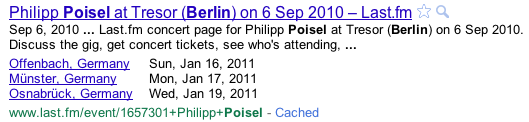
\includegraphics[width=\linewidth]{./resources/rich-snippets-poisel.png}
 \caption{Rich Snippet preview for the Philipp Poisel Concert held in Berlin on September 6th, 2010.}
 \label{fig:poisel-rich-snippet}
 \end{center}  
\end{figure}

%%%  2.3 How Much Semantic Markup is out There?  %%%
\subsection{How Much Semantic Mark-up is Out There?}                         \label{sec:how-much-markup}
Goel et al. have compiled some statistics with regards to semantic mark-up on the Web in June 2010~\cite{Goel:SemTech10}. A random sample of one million Web pages have been harvested in order to compare the use of Microformats and RDFa markup. Then, they examined how much of this mark-up data was actually used for Rich Snippets. It is remarkable and surprising how few semantic mark-up was live on the Web overall, and even more, that only a tiny fraction of all this semantic mark-up was then used for Rich Snippets at the time of their experiment. Table~\ref{tab:google-stats} shows the detailed results.

Further analysis of the dataset has shown a number of pitfalls: incorrect labeling (e.g. marking up the date of an event as part of the event description), or incorrect inclusion of unrelated words in the structured mark-up (e.g. marking up ``written by John Doe" rather than just ``John Doe" as value of the property \texttt{v:reviewer}). Furthermore, they observed a general confusion with what parts of a document should be marked up at all. Although at the time of the experiment some Web pages included RDFa event markup, none of them were used for Rich Snippets.

\begin{table}[htbp]
 \begin{center}
  \begin{tabular}{|l|l|l|}
  \multicolumn{1}{c}{\textbf{}} & \multicolumn{1}{|c}{\textbf{Microformats}} & \multicolumn{1}{|c|}{\textbf{RDFa}} \\
  \hline
  Total pages & 40,091 & 2,514 \\
  \hline
  hCard / People & 33,675 (13\%) & 1,160 \\
  \hline
  Reviews & 1,950 (88\%) & 872 (66\%) \\
  \hline
  Recipe & 152 (53\%) & -- \\
  \hline
  hCalendar / Event & 126 (41\%) & -- \\
  \hline
  Products & 519 & 77 \\
  \hline
  \end{tabular}
  \caption[One million Web pages sampled from the Internet in June 2010.]{One million Web pages sampled from the Internet in June 2010. Percentages in parenthesis: actually used for generating Rich Snippets. Source:~\cite{Goel:SemTech10}.}
  \label{tab:google-stats}
 \end{center}
\end{table}

\subsection{Google Rich Snippets Variants}
Search result snippets are the classic four line extracts of relevant sections of a website that search engines typically present to users in order to facilitate the decision of whether the page contains the desired information, or not. The more information a search result snippet can provide, the easier this decision becomes. Rich Snippets allow for more detailed extended search result snippets. Webmasters can label their websites' content to communicate that each labeled piece of mark-up represents a certain type of data: for example a person name, a business address, or a review. In the following we present the currently supported Rich Snippets.

\subsubsection{Reviews}
Review Rich Snippets can help users get a quick overview of reviewed items using a common five star rating system. Either individual reviews can be marked up (for example an editor's review of a book), or aggregate review information (for example the average rating for a restaurant). The syntax is derived from the \texttt{hReview} microformat. Figure~\ref{fig:rich-snippets-reviews} shows a concrete example of the Rich Snippet format.
\begin{figure}[htbp!]
\begin{center}
  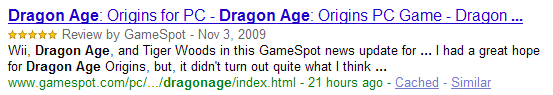
\includegraphics[width=0.75\linewidth]{./resources/rich-snippets-reviews.png}  
  \caption[Screenshot of a Rich Snippet for reviews.]{Screenshot of a Rich Snippet for reviews. Source: \url{http://www.google.com/help/hc/images/webmasters_146645_individualimage.png}.}
  \label{fig:rich-snippets-reviews}
  \end{center}  
\end{figure}

\subsubsection{People}
People Rich Snippets allow users to get more accurate information on people properties such as name, job title, or address. The syntax is derived from the \texttt{hCard} microformat. Figure~\ref{fig:rich-snippets-people} shows a concrete example of the Rich Snippet format.
\begin{figure}[htbp!]
\begin{center}
  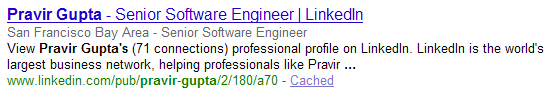
\includegraphics[width=0.75\linewidth]{./resources/rich-snippets-people.png}
  \caption[Screenshot of a Rich Snippet for people.]{Screenshot of a Rich Snippet for people. Source: \url{http://www.google.com/help/hc/images/webmasters_146676_rspeople.png}.}
  \label{fig:rich-snippets-people}
  \end{center}  
\end{figure}

\subsubsection{Events}
Events Rich Snippets help users get more details on upcoming events by listing venues, dates etc. The syntax is derived from the \texttt{hCalendar} microformat. Figure~\ref{fig:rich-snippets-events} shows a concrete example of the Rich Snippet format.
\begin{figure}[htbp!]
\begin{center}
  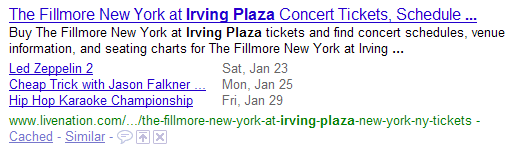
\includegraphics[width=0.75\linewidth]{./resources/rich-snippets-events.png}
  \caption[Screenshot of a Rich Snippet for events.]{Screenshot of a Rich Snippet for events. Source: \url{http://www.google.com/help/hc/images/webmasters_164506_rsevents.png}.}
  \label{fig:rich-snippets-events}
  \end{center}  
\end{figure}

\subsubsection{Recipes}
Recipes Rich Snippets serve to highlight properties of recipes such as ingredients, preparation time, or calories. The syntax is derived from the \texttt{hRecipe} microformat. Figure~\ref{fig:rich-snippets-recipes} shows a concrete example of the Rich Snippet format.
\begin{figure}[htbp!]
\begin{center}
  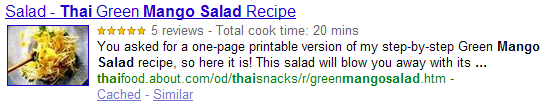
\includegraphics[width=0.75\linewidth]{./resources/rich-snippets-recipes.png}
    \caption[Screenshot of a Rich Snippet for recipes.]{Screenshot of a Rich Snippet for recipes. Source: \url{http://www.google.com/help/hc/images/webmasters_173379_en.png}.}
  \label{fig:rich-snippets-recipes}
  \end{center}  
\end{figure}

\subsubsection{Products}
Products Rich Snippets can help users get an overview on products ratings, prices, or availabilities. There are several options to mark up products, among them GoodRelations~\cite{Hepp:GoodRelations} and the \texttt{hProduct} microformat. Figure~\ref{fig:rich-snippets-products} shows a concrete example of the Rich Snippet format.
\begin{figure}[htbp!]
\begin{center}
  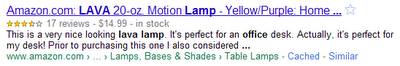
\includegraphics[width=0.75\linewidth]{./resources/rich-snippets-products.png}
    \caption[Screenshot of a Rich Snippet for products.]{Screenshot of a Rich Snippet for products. Source: \url{http://www.google.com/help/hc/images/webmasters_1095551_en.png}.}
  \label{fig:rich-snippets-products}
  \end{center}  
\end{figure}

\subsubsection{Organizations}
Organizations Rich Snippets are used in combination with other structured mark-up such as events or reviews markup to detail business addresses, telephone numbers, or geographic location. Figure~\ref{fig:rich-snippets-organizations} shows a concrete example of the Rich Snippet format.
\begin{figure}[htbp!]
\begin{center}
  
\includegraphics[width=0.75\linewidth]{./resources/rich-snippets-organizations.png}
    \caption[Screenshot of a Rich Snippet for organizations.]{Screenshot of a Rich Snippet for organizations. Source: \url{http://www.seomoz.org/img/upload/hevent-snippet.png}.}
  \label{fig:rich-snippets-organizations}
  \end{center}  
\end{figure}

\subsubsection{Breadcrumbs}
Breadcrumb Rich Snippets are an experimental feature that allow users to navigate and understand a website's link hierarchy. There can be more than one breadcrumb trails. Figure~\ref{fig:rich-snippets-breadcrumbs} shows a concrete example of the Rich Snippet format.
\begin{figure}[htbp!]
\begin{center}
  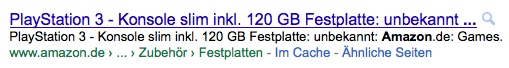
\includegraphics[width=0.75\linewidth]{./resources/rich-snippets-breadcrumbs.jpg}
    \caption[Screenshot of a Rich Snippet for breadcrumbs.]{Screenshot of a Rich Snippet for breadcrumbs. Source: \url{http://www.macseoblog.de/wp-content/uploads/2011/05/breadcrumb-rich-snippet-serps.jpg}.}
  \label{fig:rich-snippets-breadcrumbs}
  \end{center}  
\end{figure}

\subsubsection{Videos}
Videos Rich Snippets can help users discover video content more quickly on websites. There are two mark-up formats supported, namely Facebook's Like\footnote{\url{https://developers.facebook.com/docs/reference/plugins/like/}} button mark-up and Yahoo!'s SearchMonkey RDFa\footnote{\url{http://developer.search.yahoo.com/help/objects/video}} mark-up. Figure~\ref{fig:rich-snippets-videos} shows a concrete example of the Rich Snippet format.
\begin{figure}[htbp!]
\begin{center}
  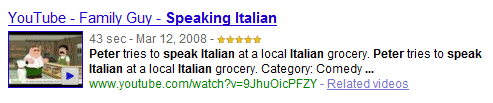
\includegraphics[width=0.75\linewidth]{./resources/rich-snippets-videos.png}
    \caption[Screenshot of a Rich Snippet for videos.]{Screenshot of a Rich Snippet for videos. Source: \url{http://www.seomoz.org/img/upload/gg-rich-snippets-3.gif}.}
  \label{fig:rich-snippets-videos}
  \end{center}  
\end{figure}

\subsection{Nesting Different Rich Snippets Variants}
One of the advantages of structured mark-up is that it can be easily nested. A section that marks up a reviewed item can, for example add more details about the reviewing entity by intermixing persons mark-up, or organizations mark-up. Figure~\ref{code:rich-snippet-nested} shows a concrete example of nested mark-up.

\begin{figure}[htbp!]
\begin{center}
{\footnotesize
\begin{code}
<div xmlns:v="http://rdf.data-vocabulary.org/#"
     typeof="v:Review">
  <div rel="v:itemreviewed">
    <span typeof="Organization">   
      <span property="v:name">L'Amourita Pizza</span>
      Located at 
      <span rel="v:address">
        <span typeof="v:Address">
          <span property="v:street-address">123 Main St</span>, 
          <span property="v:locality">Albuquerque</span>, 
          <span property="v:region">NM</span>.
        </span>
      </span>
      <a href="http://pizza.example.com/" rel="v:url">
        http://pizza.example.com
      </a>
    </span>
  </div>
  Reviewed by 
  <span property="v:reviewer">Bob Smith</span>. 
  Rated: 
  <span rel="v:rating">
    <span property="v:value">9</span>/
    <span property="v:best">10</span> (Excellent)
  </span>
</div> 
\end{code}}
  \caption[RDFa markup showing nesting of review and organization mark-up.]{RDFa markup showing nesting of review and organization mark-up. The reviewed item is a restaurant. Its location is given in organization mark-up form in a nested way.}
  \label{code:rich-snippet-nested}
  \end{center}  
\end{figure}

\subsection{The Rich Snippets Testing Tool}
Google provides a Rich Snippets testing tool, which allows for webmasters to check their structured markup and assure that the search engine can extract the structured data from webpages. The tool generates a preview of how a Rich Snippet based on the structured data on a webpage might look like, and also lists the data it could extract. Figure~\ref{fig:rich-snippets-testing-tool} shows a preview for the structured recipe data as found on \url{www.foodnetwork.com/recipes/banana-bread-recipe/index.html} (retrieved on May 10, 2011).

\begin{figure}[htbp!]
\begin{center}
  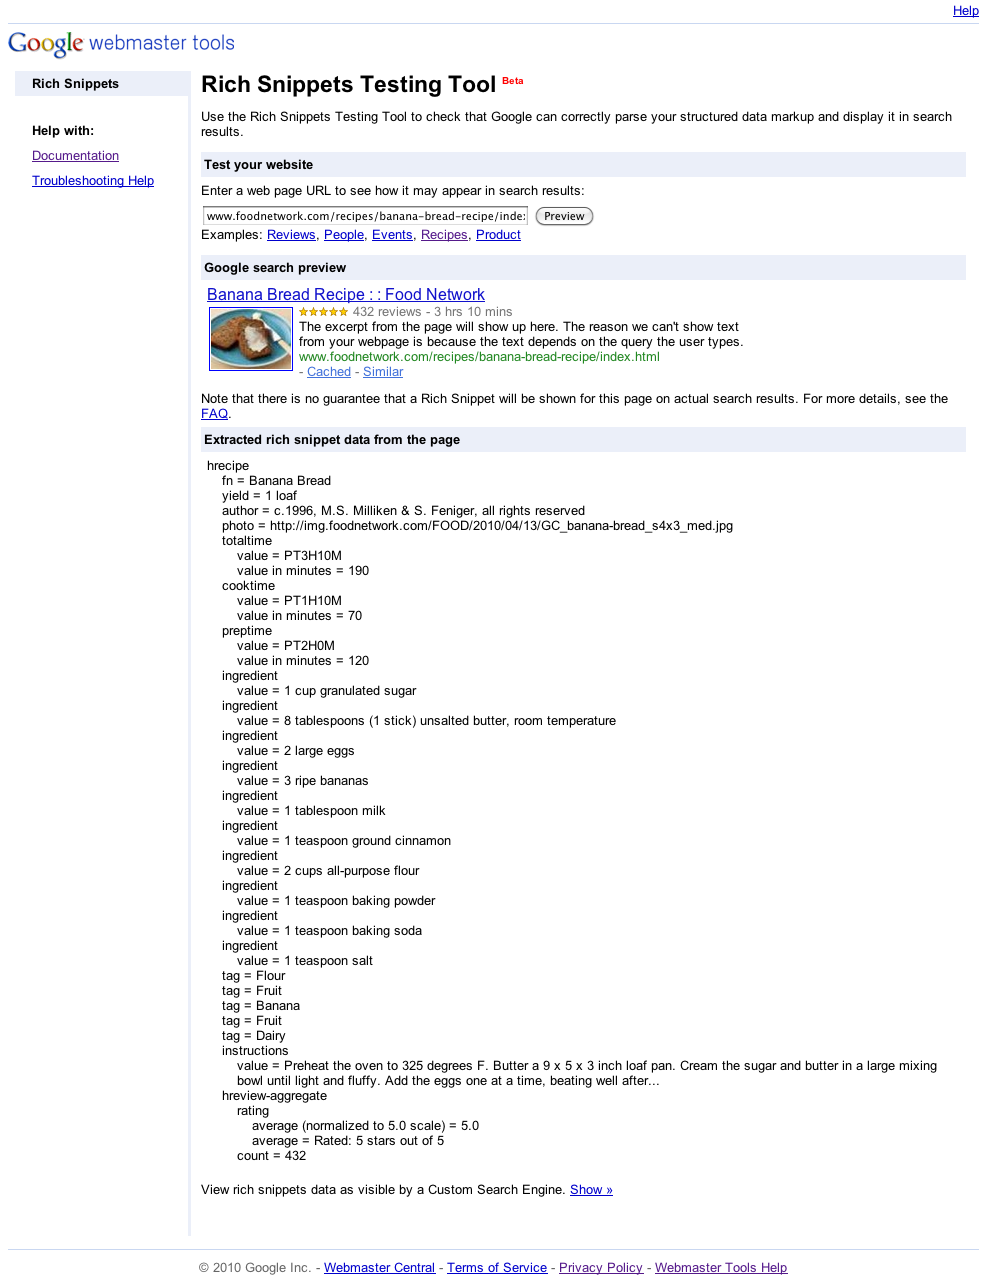
\includegraphics[width=1.0\linewidth]{./resources/rich-snippets-testing-tool.png}
    \caption{Screenshot of the Rich Snippets testing tool showing a recipe Rich Snippet preview.}
  \label{fig:rich-snippets-testing-tool}
  \end{center}  
\end{figure}

In the following Section we introduce ways to add structure to unstructured textual data.

\section{Structuring Unstructured Textual Data}
When we speak of adding structure to unstructured textual data we mean the process of extracting the main concepts in the form of named entities from a given text. An ``entity" is defined\footnote{\url{http://wordnetweb.princeton.edu/perl/webwn?s=entity}} by WordNet as ``that which is perceived or known or inferred to have its own distinct existence (living or nonliving)". Typically named entities from a text can be persons, companies, organizations, geographies, but also things like quantities, expressions of time, books, albums, authors etc. The extraction is based on Natural Language Processing (NLP) and Machine Learning.

\subsection{Natural Language Processing Services}\label{sec:nlp-services}
Natural Language Processing is defined\footnote{\url{http://wordnetweb.princeton.edu/perl/webwn?s=natural\%20language\%20processing}} as ``the branch of information science that deals with natural language information". From the many NLP toolkits, in the following we list some NLP Web services that link to datasets in the LOD cloud described in Section~\ref{sec:lodcloud} in order to disambiguate named entities.

\subsubsection{OpenCalais}\label{sec:opencalais}
OpenCalais~\cite{OpenCalais} is the only Web service we use that provides details on occurrences in concrete sections of the submitted coherent text. This allows for exact matching of the location in the text where a certain entity is believed to appear. This is especially useful as OpenCalais is also oftentimes capable of recognizing references within the text to prior discovered entities (see the emphasized words as an example: ``\emph{Obama} thanked people for their work in ensuring the victory. \emph{He} also thanked his family […]"). An OpenCalais response consists of three parts:

\begin{itemize}
\item a list of overall topics that the text could be categorized in.
\item a list of concrete entities that occur in the text.
\item a list of social tags that a human being might assign to the text.
\end{itemize}

The problem with the extracted entities is that they are not always disambiguated. An example is the URI \url{http://d.opencalais.com/pershash-1/cf42394f-4ae9-3e8e-958a-088149c86565.html} that represents the concept of type ``person" of Barack Obama. However, president Barack Obama is also represented by the URI \url{http://d.opencalais.com/pershash-1/cfcf1aa2-de05-3939-a7d5-10c9c7b3e87b.html} that was returned in one and the same response to one of our test requests. A second issue is that only a tiny fraction of the returned entities link to other Linked Open Data (LOD) sources in the LOD cloud. In order to find links to the linking hub DBpedia, each returned entity has to be retrieved at the expense of an HTTP request, and the returned RDF has to be checked for said links.

\subsubsection{AlchemyAPI}
AlchemyAPI~\cite{AlchemyAPI} differentiates between entities and concepts, however, in practice the difference being very subtle, we can treat entities and concepts the same. Overall the AlchemyAPI results are very accurate and of mostly excellent Linked Data quality as there are links to well-known members of the LOD cloud, among others to DBpedia, OpenCyc, and Freebase. AlchemyAPI also provides links to other data sources, however, sometimes the returned URIs resolve to 404 ``Not found" errors (one example that we came across during our tests was the URI \url{http://umbel.org/umbel/ne/wikipedia/George_W._Bush.rdf}, which should represent the concept of the person George W. Bush). AlchemyAPI also oftentimes returns very related, but not directly relevant entities.

\subsubsection{Zemanta}
Zemanta~\cite{Zemanta} provides high quality entities that are linked to well-known members of the LOD cloud, e.g. DBpedia, Semantic CrunchBase, or Freebase. Zemanta convinces through very accurate entity disambiguation. We could not find any evident problem with the service, except for the sometimes relatively small number of entities, where the other services we use offer more.

\subsubsection{DBpedia Spotlight}
DBpedia Spotlight~\cite{spotlight} is a tool for annotating mentions of DBpedia resources in text, providing a solution for linking unstructured information sources to the Linked Open Data cloud through DBpedia. DBpedia Spotlight performs named entity extraction, including entity detection and disambiguation with adjustable precision and recall.

\subsection{URI Lookup Services}\label{sec:uri-lookup-services}
When we say \textit{URI lookup} we mean the process of mapping a term to an entity identified by a URI that represents this term. For example when talking about the US president, the term \texttt{barack obama} can be related to the entity identified by the URI \url{http://dbpedia.org/resource/Barack_Obama}. The main problem
with URI lookup is its ambiguity as terms are taken out of context. Hence, the term \texttt{philadelphia} can
refer to the concept of the city of Philadelphia, PA, or to the cream cheese by Kraft Foods.

We have tested several URI lookup services independently. Each has its particular pros and cons, as outlined in each service's Section. We found that we can get the best results if we combine the results from the particular services using a simple majority-based voting system to determine a combined final result.

\subsubsection{DBpedia Lookup}
DBpedia Lookup~\cite{kobilarov} is a URI lookup service for DBpedia initially developed by Georgi Kobilarov. It returns results in the \texttt{http://dbpedia.org/\-resource/\-\{Thing\}} namespace.

\subsubsection{Freebase}
Freebase~\cite{NYTimes:Freebase} is an entity graph of people, places and things with a URI lookup service. Freebase is owned by Google~\cite{metaweb}, however, was developed by Metaweb before. It returns results in the \texttt{http://rdf.freebase.com/ns/\-\{Language\}/\{Thing\}} namespace.

\subsubsection{Sindice}
Sindice~\cite{Tummarello:Sindice} is a joint research project by DERI, Fondazione Bruno Kessler, and OpenLink software. It provides a URI lookup service that returns results from any namespace.

\subsubsection{Uberblic}
Uberblic~\cite{Kobilarov:Uberblic} is an integration service for data on the Web by Uberblic Labs, developed and founded by Georgi Kobilarov. It also provides a URI lookup service that returns results from the namespace
\texttt{http://uberblic.org/\-resource/\{Thing\}}.

In the following Section we show how URI lookup services and NLP services can be used to enrich social network communication.

\section{Enriching Social Network Communication}
In this Section we show how social network communication can be enriched on-the-fly using extension or plug-in mechanisms of modern Web browsers. We use the Google Chrome~\cite{google:chrome} browser and its extension mechanism as representative example.

For data aggregation, we show how common Web analytics software can be used in combination with extension mechanisms of Web browsers to track socially enriched network communication. We use Google Analytics~\cite{analytics} as a common free Web analytics software. 

\subsection{Google Chrome Extensions Architecture}
Google Chrome extensions\footnote{\url{http://code.google.com/chrome/extensions/index.html}} are small software programs that can be installed to enrich the browsing experience with the Google Chrome browser. They are written using a combination of standard Web technologies, such as HTML, JavaScript, and CSS. Chrome extensions get usually (but not necessarily) distributed through the Chrome Web Store\footnote{\url{https://chrome.google.com/webstore/}}. There are several types of extensions, for our experiment we focused on extensions based on so-called content scripts. Content scripts are JavaScript programs that run in the context of Web pages via dynamic code injection, similar to the Firefox Greasemonkey extension\footnote{\url{http://www.greasespot.net/}}. By using the standard Document Object Model (DOM), they can read or modify details of the Web pages a user visits. An example of such modification is, e.g. removing background images for better legibility. Content scripts can run on any website, or be limited to just certain websites. This can be controlled by the extension developer with a so-called manifest file in JSON format. When a user installs an extension, the access rights of the extension are displayed and must be acknowledged by the user.

\subsection{Using Google Analytics for Data Aggregation}\label{sec:analytics}
Google Analytics\footnote{\url{http://www.google.com/analytics/}} is Google's Web analysis solution that allows for detailed statistics about the visitors of a website. The software is implemented by adding an invisible snippet of JavaScript code on the to-be-tracked pages of a website. This code collects visitor data through a request for a specific 1~x~1 pixel image on Google's servers, during which page data and user data are reported in the query part of the image's URL. In addition to that the snippet sets a first party cookie on visitors' computers in order to store anonymous information such as the timestamp of the current visit, whether the visitor is a new or returning visitor, and the referrer of the website that the visitor came from. Part of the shared visitor information is the IP address, which allows for IP-based geolocation.

\subsection{Twitter Swarm NLP}
We have developed a Google Chrome extension called Twitter Swarm NLP\footnote{\url{https://chrome.google.com/webstore/detail/dpbphenfafkflfmdlanimlemacankjol}} that injects JavaScript code via a content script into the Twitter.com homepage. By installing this extension, users explicitly opt-in to their data as a Twitter.com visitor being tracked by Google Analytics. The extension first checks if the user is logged in to Twitter.com, and if so, retrieves the tweets of the current user's timeline (\url{http://twitter.com/#}), or search result page (e.g. \url{http://twitter.com/#!/search/%23semweb}), or profile page (e.g. \url{http://twitter.com/#!/timberners_lee}) on a one-by-one basis, and performs Named Entity Extraction (NEE) via Natural Language Processing (NLP) using remote NLP Web services on each of the tweets. The extracted entities are then displayed below each tweet on the Twitter.com homepage, as shown in Figure~\ref{fig:danbri}, and are then sent to Google Analytics for further processing.

\begin{figure}[htbp!]
\begin{center}
  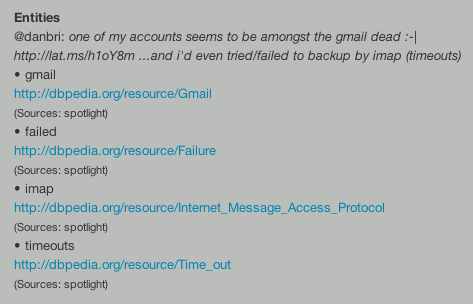
\includegraphics[width=0.56\linewidth]{./resources/twitter-swarm-nlp-danbri.png}
    \caption{Screenshot of the original tweet above, and the thereof extracted entities below.}
  \label{fig:danbri}
  \end{center}  
\end{figure}

In the following Section we introduce Media Fragments URIs that allow for fine-grained in-media links.

\section{Media Fragments URIs}
The Media Fragments URIs~\cite{W3C:MediaFrags} W3C Working Draft specifies the syntax for constructing media fragment URIs and explains how to handle them when used over the HTTP~\cite{fielding1999hypertext} protocol. The syntax is based on the specification of particular name-value pairs that can be used in URI~\cite{bernerslee2005uri} fragment and URI query requests to restrict a media resource to a certain fragment. Before the introduction of the \texttt{video} and \texttt{audio} elements in HTML5~\cite{w3c_html5}, audio and video resources on the World Wide Web were treated as ``foreign" objects, which could only be embedded using plug-ins such as the Adobe Flash Player\footnote{\url{http://get.adobe.com/flashplayer/}} that is capable of decoding and interacting with the media resource. With the \texttt{video} and \texttt{audio} elements, both video and audio resources are now treated like first class citizens, however, support for fragments of these resources is still impossible. Currently there is no way to embed only the first half hour of a two-hour keynote recording. Specific media servers are required to provide for server-side features such as direct access to time offsets into a video, or sub-resources of an audio file without the need to retrieve the entire resource. The Media Fragments URIs W3C Working Draft specification provides for a media-format independent standard means of addressing media fragments on the Web using Uniform Resource Identifiers (URI). The specification regards media fragments along four different dimensions: temporal, spatial, named, and tracks. While the specified addressing schemes apply to video and audio resources, the spatial fragment addressing may also be used on images. All dimensions are logically independent and can be combined. The outcome is independent of the order of the dimensions.

\subsection{Use Cases}
Media Fragments URIs can be used to efficiently share video or audio fragments via social networks or email. In addition to that Media Fragments URIs can also be automatically created by search engines in order to provide deep-links into multimedia resources. A different use case is the annotation of multimedia resources with RDF~\cite{RDF}. In the following we give an overview of the four dimensions, as  defined by the specification, and have a look at URI fragments and URI queries before.

\subsection{URI Fragments and Queries}
Every URI is defined in RFC 3986~\cite{bernerslee2005uri} as consisting of the following four parts:\\

\noindent  \texttt{<scheme> : <hierarchical part> [ ? <query> ] [ \# <fragment> ]}\\

\noindent  There are therefore two possibilities for representing a media fragment in URIs: the URI query part, or the URI fragment part. The main difference between a URI query and a URI fragment is that a URI query produces a new resource, while a URI fragment provides a secondary resource of the same media type as the main resource, to which it has a direct relationship. URI fragments are resolved from the primary resource without another request to the server. In contrast, URI queries always require a new retrieval action, even if the main resource has been retrieved before. An example of a URI fragment used to address a media fragment is \texttt{http://www.example.org/video.ogv\-\#t=60,100}. The primary resource in this case is thus \texttt{http://www.ex\-ample.org/video.ogv}, and the URI fragment is \texttt{\#t=60,100}, which corresponds to the seconds 60 to 100 of the whole primary resource.

\subsection{Media Fragments Dimensions}
As outlined before, the Media Fragments URIs specification regards media fragments along four different dimensions. In the following we will have a closer look at these dimensions, and show example Media Fragments URIs that use them.

\subsubsection{Temporal Dimension}
This dimension denotes a specific time range in the original media, such as ``starting at second 10, continuing until second 20". Temporal clipping is denoted by the name \texttt{t}, and specified as an interval with a start time and an end time. Either or both may be omitted, with the start time defaulting to 0 seconds and the end time defaulting to the duration of the source media. The interval is half-open: the start time is considered part of the interval, whereas the end time is considered to be the first time point that is not part of the interval. If only a single number is given, this corresponds to the start time, except if it is preceded by a comma, which would in this case indicate the end time. Supported time formats are Normal Play Time (\texttt{npt:}, default) as defined in RFC 2326~\cite{rfc2326}, SMPTE timecodes~\cite{smpte} (\texttt{smpte:}), or real-world clock time (\texttt{clock:}), also defined in RFC 2326~\cite{rfc2326}. Some examples, taken from~\cite{W3C:MediaFrags}, are given below:\\

\texttt{t=10,20} Results in the time interval [10,20).\\
\indent \texttt{t=,20} Results in the time interval [0,20).\\
\indent \texttt{t=10} Results in the time interval [10,end).

\subsubsection{Spatial Dimension}
This dimension denotes a specific range of pixels in the original media, such as ``a rectangle with size (100, 100) with its top-left at coordinate (10, 10)". Spatial clipping selects a rectangular area of pixels from videos or images. The rectangle can be specified as pixel coordinates or percentages. The selection is denoted by the name \texttt{xywh}. The value is either of the two formats \texttt{pixel:} (default) or \texttt{percent:} and four comma-separated integers. The integers denote x, y, width, and height. With pixels coordinates, x=0, y=0 refer to the top left corner of the image. With percentage coordinates, x and width are interpreted as a percentage of the width of the original media, and y and height are interpreted as a percentage of the original height. Some examples, taken from~\cite{W3C:MediaFrags}, are given below:\\

\texttt{xywh=160,120,320,240} Results in a 320x240 box at x=160, y=120.\\
\indent \texttt{xywh=pixel:160,120,320,240} Results in a 320x240 box at x=160, y=120.\\
\indent \texttt{xywh=percent:25,25,50,50} Results in a 50\%x50\% box at x=25\%, y=25\%.

\subsubsection{Named Dimension}
This dimension denotes a named temporal fragment within the original media, such as ``chapter 2", and can be seen as a convenient way of specifying a temporal fragment. In consequence a named fragment can always be resolved to a temporal fragment. Name-based selection is denoted by the key name \texttt{id}, the value is a percent-encoded string. As with track selection defined in the next Section, determining which names are valid requires knowledge of the original media item. Some examples, taken from~\cite{W3C:MediaFrags}, are given below:\\

\texttt{id=1} Results in only extracting the section ``1".\\
\indent \texttt{id=chapter-1 } Results in only extracting the section ``chapter-1".\\
\indent \texttt{id=Radio\%20Edit} Results in only extracting the section ``Radio Edit".

\subsubsection{Track Dimension}
This dimension denotes one or more tracks in the original media, such as ``the English audio and the video track". Track selection allows the extraction of tracks (audio, video, subtitles, etc.) from a media container that supports multiple tracks. Track selection is denoted by the name \texttt{track}. The value is a percent-encoded string. As the allowed track names are determined by the original source media, this information has to be known beforehand. Some examples, taken from~\cite{W3C:MediaFrags}, are given below:\\

\texttt{track=1} Results in only extracting track 1.\\
\indent \texttt{track=vid\&track=sub} Results in extracting track ``vid" and track ``sub".\\
\indent \texttt{track=Wide\%20Angle} Results in only extracting track ``Wide Angle".\\

\noindent In the following Section we show how Media Fragments URIs can be used to annotate videos on a video platform such as YouTube.

\section{SemWebVid -- RDF Video Annotation}
SemWebVid\footnote{\url{http://tomayac.com/semwebvid/}}~\cite{semwebvid} is a Web application that allows for the automatic on-the-fly generation of Resource Description Framework (RDF) video descriptions. These descriptions are based on two pillars: first, on a combination of user-generated metadata for a video such as title, summary, and tags; and second, on closed captions, which can be user-generated, or be auto-generated via audio transcription services. This textual information is enriched using multiple Natural Language Processing (NLP) Web services in parallel in order to extract named entities. The resulting named entities are then merged, and wherever possible the detected named entities are matched back to concepts represented by URIs in the sense of Linked Data. The final result is a downloadable RDF description of the video. At present the application is interactive, i.e. requires user interaction in order to create an RDF video description, however, there is also a command line version available, so that the process could be automated and become a regular part of video crawling techniques used by general search engines. A screenshot of SemWebVid can be seen in Figure~\ref{fig:semwebvid}. The overall data flow of the application can be seen in Figure~\ref{fig:dataflow}.

\begin{figure}[htbp!]
\begin{center}
  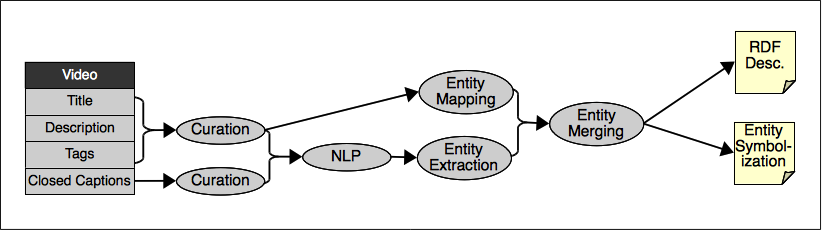
\includegraphics[width=\linewidth]{./resources/semwebvid-dataflow.png}
    \caption{SemWebVid Dataflow Diagram.}
  \label{fig:dataflow}
  \end{center}  
\end{figure}

\subsection{Entity Extraction and URI Lookup}
In the following we present how SemWebVid handles URI lookup (for tags) and entity extraction (for closed captions).

\subsubsection{URI Lookup for Tags}
We try to map the list of tags back to URIs using plaintext URI lookup Web services, as outlined in Section~\ref{sec:uri-lookup-services}. The different services do not necessarily always agree on the same entity for a given term. It is thus very important to preserve provenance data in order to judge and estimate the quality of the looked-up URIs.

\subsubsection{Entity Extraction for Closed Captions, Title, Description}
With regards to the closed captions, description, and title we work with NLP entity extraction Web services, as outlined in Section~\ref{sec:nlp-services}. In our experiments we found that including the tags as a comma-separated list greatly helps in directing the NLP engines in the right direction. We had best results with the concatenation (in this order) of: title, description, comma-separated list of tags, and closed captions. In addition to that we also found that only a combination of all NLP Web services turned out satisfying results.

\subsection{Entity Depiction}\label{sec:depiction}
In a final step the detected entities from the different NLP Web services are merged, and a symbolization or depiction for each entity gets retrieved by means of a heuristic approach, including Google image search~\cite{googleimg}. Potential depiction candidates get extracted from the Linked Open Data cloud. We use \texttt{foaf:depiction} for DBpedia, and \texttt{<http://rdf.\-freebase.com\-/ns/common.topic.image>} for Freebase URIs. Because of the current DBpedia being based on Wikipedia snapshots, sometimes image sources are no longer valid. However, as the filenames used on Wikipedia are very identifying, a simple Google image search for the filename usually returns the image in question. See Figure~\ref{fig:depiction} for an example of such entity depictions.

\begin{figure}[htbp!]
\begin{center}
  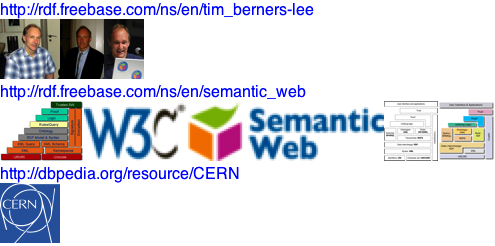
\includegraphics[width=0.65\linewidth]{./resources/semwebvid-depiction.png}
    \caption{Depiction of entities (Tim Berners-Lee, Semantic Web, etc.).}
  \label{fig:depiction}
  \end{center}  
\end{figure}

\subsection{Linkable RDF Video Descriptions}
Each RDF video description that gets generated for a video has its separate video-dependent URI, which allows for deep-linking of video descriptions. This means that the state of the application can be passed to a different user agent. For example the URI \url{http://tomayac.com/semwebvid/#id=3PuHGKnboNY} links to the application state of the SemWebVid application where an on-the-fly RDF video description of Barack Obama's inauguration speech gets generated.

\subsection{In-Video Links Using Media Fragment URIs}
SemWebVid uses Media Fragments URIs to link to fragments of video content that were introduced by the W3C Media Fragments Working Group~\cite{W3C:MediaFrags}. For example \url{http://tomayac.com/semwebvid/#id=3PuHGKnboNY;t=10} links to the scene 10 seconds in the video of Obama's inauguration speech where Obama starts repeating the inauguration oath.

\subsection{Color-coded Provenance}\label{sec:provenance}
In SemWebVid we introduce a novel way of visually representing provenance data. The problem is that an entity can be detected by more than one source, for example in the phrase ``I, Barack Hussein Obama, do solemnly swear that I will execute the office of President to the United States faithfully", the entity ``Barack Hussein Obama" represented by the URI \url{http://dbpedia.org/resource/Barack_Obama} gets recognized by all NLP Web services. By means of partial background highlighting in different colors we can represent up to four sources for one entity. Figure~\ref{fig:provenance} shows the provenance color-coded representation of the entity ``United States" simultaneously detected by AlchemyAPI (highlighted in red) on the left, and by OpenCalais (highlighted in yellow). In addition to that the OpenCalais URI was found to be \texttt{owl:sameAs} to a DBpedia URI, coming from Sindice (highlighted in orange).

\begin{figure}[htbp!]
\begin{center}
  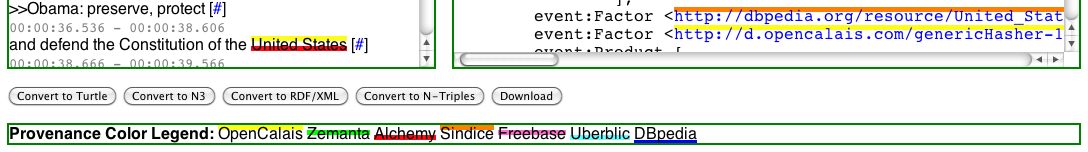
\includegraphics[width=\linewidth]{./resources/semwebvid-provenance.png}
    \caption[Two entities provenance color-coded.]{Two entities provenance color-coded. The provenance color legend is below.}
  \label{fig:provenance}
  \end{center}  
\end{figure}

In the next Section we give an outlook on future work, and open research questions to be treated in our thesis.

\section{Evaluation and Future Work}
In this Section we present our already happened and upcoming evaluation, and also give an outlook on future work. Our objective for this thesis is to create a framework that allows for the semi-automatic generation of summaries or compilations of several pieces of media content covering a certain event. The term ``event" is defined\footnote{\url{http://wordnetweb.princeton.edu/perl/webwn?s=event}} by WordNet as ``something that happens at a given place and time". A concrete example for such event can thus be a keynote speech given at a conference, where media content is published on social networks while the event is still going on. This includes people taking pictures or videos with their mobile phones or digital cameras that are then (the network permitting) immediately shared on social networks in order to allow for their followers and friends to get a feeling for the event's atmosphere, or simply for documentation purposes in the sense of a (public) diary. The process of generating a summary or compilation for an event includes the following steps:

\begin{description}
\item [Event-Selection:] Decide on an event that shall be summarized.
\item [Micropost-Annotation:] Find relevant microposts on social networks containing links to media content about the event, and annotate the microposts one by one using RDF, leveraging data from the LOD cloud.
\item [Media-Content-Annotation:] Retrieve the pieces of media content and the accompanying metadata one by one, and annotate them using RDF, leveraging data from the LOD cloud.
\item [Media-Content-Ranking:] Rank and order the pieces of media content by relevance, creation time, duration, and other criteria.
\item [Media-Content-Compilation:] Based on the ranking, suggest a summary or compilation taking into account user constraints such as desired duration, composition (videos only, images only, combination of both), etc.
\end{description}

\subsection{Evaluation}
In the following we introduce our evaluation plan and present already existing evaluation for each of these steps.

\subsubsection{Event-Selection}
For this task we currently have preliminary results only. We have selected two recent events, the Semantic Technology Conference 2011 in San Francisco, CA (SemTech)~\cite{semtech}, and the Apple Worldwide Developers Conference 2011 (WWDC)~\cite{wwdc}, also in San Francisco. For WWDC there is a DBpedia page (\url{http://dbpedia.org/resource/Apple_Worldwide_Developers_Conference}), for SemTech there is just the generic event landing page (\url{http://semtech2011.semanticweb.com/}). We have disambiguated both event names with their locations using the API that powers both our Twitter Swarm NLP and Facebook Swarm NLP Chrome extensions, which are described in detail in Sections~\ref{fb-swarm} and~\ref{tw-swarm}. The results can be seen in Figures~\ref{code:wwdc} and~\ref{code:semtech}. For WWDC the plaintext labels of the named entities are ``Apple", ``San Francisco", ``Apple Inc.", ``iPhone OS", and ``Apple Worldwide Developers Conference". Each named entity is uniquely identified by a URI in the LOD cloud, which allows for ambiguity-free exploration of related entities. This is very important for the discovery of microposts on social networks in the task \emph{Micropost-Annotation} that might have links to media content, especially in cases where no unique hashtag is known.

\begin{figure}[htbp!]
\begin{center}
{\footnotesize
\begin{code}
[
    \{
        "name": "Apple",
        "uris": [
            \{
                "uri": "http://dbpedia.org/resource/Apple_Inc."
            \}
        ]
    \},
    \{
        "name": "San Francisco",
        "uris": [
            \{
                "uri": "http://dbpedia.org/resource/San_Fran-
                        cisco,_California"         
            \}
        ]
    \},
    \{
        "name": "Apple Inc.",
        "uris": [
            \{
                "uri": "http://dbpedia.org/resource/Apple_Inc."         
            \}
        ]
    \},
    \{
        "name": "IPhone OS",
        "uris": [
            \{
                "uri": "http://dbpedia.org/resource/IPhone_OS"
            \}
        ]
    \},
    \{
        "name": "Apple Worldwide Developers Conference",
        "uris": [
            \{
                "uri": "http://dbpedia.org/resource/Apple_World-
                        wide_Developers_Conference"
            \}
        ]
    \}
]
\end{code}}
  \caption[Extracted named entities and related named entities for the WWDC conference.]{Extracted named entities and related named entities for the WWDC conference (shortened for legibility).}
  \label{code:wwdc} 
  \end{center}  
\end{figure}

\begin{figure}[htbp!]
\begin{center}
{\footnotesize
\begin{code}
[
    \{
        "name": "San Francisco",
        "uris": [
            \{
                "uri": "http://dbpedia.org/resource/San_Fran-
                        cisco,_California"
            \}
        ]
    \},
    \{
        "name": "California",
        "uris": [
            \{
                "uri": "http://dbpedia.org/resource/California"
            \}
        ]
    \},
    \{
        "name": "SEMTECH Semantic Technology",
        "uris": [
            \{
                "uri": "http://d.opencalais.com/genericHasher-1-
                        /63f3fece-56d6-3dbb-8940-cbddae9a135e"
            \}
        ]
    \},
    \{
        "name": "San Francisco, CA",
        "uris": [
            \{
                "uri": "http://dbpedia.org/resource/San_Fran-
                        cisco"
            \}
        ]
    \}
]
\end{code}}
  \caption[Extracted named entities and related named entities for the SemTech conference.]{Extracted named entities and related named entities for the SemTech conference (shortened for legibility).}
  \label{code:semtech} 
  \end{center}  
\end{figure}

\subsubsection{Micropost-Annotation}
We have implemented a generic framework for the on-the-fly enrichment of social network microposts. This framework has been successfully tested on overall 92 seven-day active users (as of June 22, 2011) of our two Chrome extensions described in Sections~\ref{fb-swarm} and~\ref{tw-swarm}. The context of the tests was the detection of news trends in microposts, Figure~\ref{fig:overtime-edge-a} shows an example. As outlined in Section~\ref{sec:analytics}, by using Google Analytics named entity occurrences can be easily tracked over time. As an example, Figure~\ref{fig:overtime-edge-b} shows the occurrences graph generated by Analytics of the named entity ``tsunami". Japan was hit by an earthquake followed by a tsunami on March 11, exactly where the peak is on the graph. In general the occurrences graphs also for other examples indeed correspond to what we would expect from the news headlines of the considered days, albeit the data is at this point not statistically significant. A more detailed evaluation can be found in~\cite{twittertrends}.

\begin{figure}[htb!]
  \begin{center}
\subfloat[Screenshot of a tweet, and a thereof extracted named entity ``gmail" with its representing DBpedia URI.]{\label{fig:overtime-edge-a}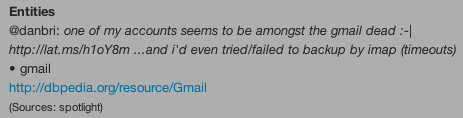
\includegraphics[width=0.46\textwidth]{./resources/twitter-swarm-nlp-tweet.png}}
\hspace{5pt}
\subfloat[Popularity of the named entity ``tsunami" from March 10 - 14. Japan was hit by a tsunami on March 11, at the peak.]{\label{fig:overtime-edge-b}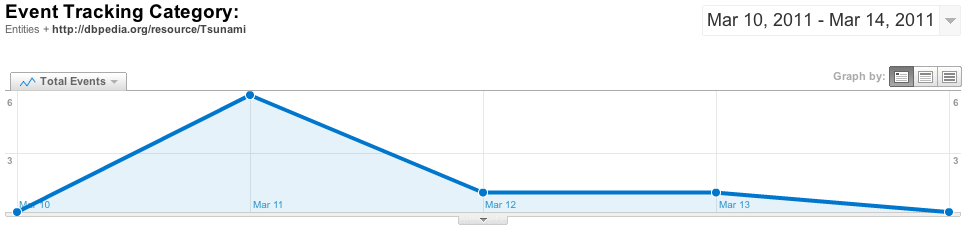
\includegraphics[width=0.47\textwidth]{./resources/twitter-swarm-nlp-tsunami.png}}
  \caption{Twitter Swarm NLP sample output and popularity of a named entity over time.}
  \label{fig:overtime}
  \end{center}  
\end{figure}

\subsubsection{Media-Content-Annotation}
For this task we currently have preliminary results only. At present we have implemented an interactive Ajax application called SemWebVid that allows for the automatic annotation of videos on YouTube with RDF, which is described in more detail in Section~\ref{sec:semwebvid}. Based on the same API that powers SemWebVid, we have implemented a command line version of the annotation mechanism that in the future can be used to batch-process videos. For now, we have annotated videos with the interactive Ajax application, and reviewed the annotations manually, however, at this point have not yet compared the annotations to a gold standard. In the current SemWebVid implementation, we use \texttt{event:factor}, \texttt{event:product}, and \texttt{event:agent} from the Event Ontology~\cite{Raimond:Event} to relate events to factors (non-person entities), products (the particular closed caption cues), and agents (persons entities). Figure~\ref{code:c64} shows a sample video fragment annotated with the Event Ontology.

\begin{figure}[htbp!]
\begin{center}
{\footnotesize
\begin{code} 
<http://gdata.youtube.com/[\ldots]/hzFp3rovfY0> event:Event :captionEvent22.
:captionEvent22
  a event:Event;
  event:time [
    tl:start "PT0.171S"^^xsd:duration;
    tl:end "PT0.177S"^^xsd:duration;
    tl:duration "PT0.006S"^^xsd:duration;
    tl:timeline :timeline;
    ];
  event:Factor <http://rdf.freebase.com/ns/en/commodore\_64>;
  event:Factor <http://dbpedia.org/resource/Commodore\_64>;
  event:Factor <http://mpii.de/yago/resource/Commodore\_64>;
  event:Factor <http://dbpedia.org/resource/Timbaland>;
  event:Factor <http://mpii.de/yago/resource/Timbaland>;
  event:Product [
    a bibo:Quote;
    rdf:value """On the Timbaland produces song Do It, the Commodore 64
                 can clearly be heard from the background."""@en;
    ].
\end{code}}
  \caption[Annotated sample video fragment.]{Annotated sample video fragment of the YouTube \url{http://www.youtube.com/watch?v=hzFp3rovfY0}. The video is about the music artist Timbaland being accused of stealing a music tune from the Commodore 64 scene. Extracted named entities in this scene are ``Timbaland" with the URI \url{http://dbpedia.org/resource/Timbaland} and ``Commodore 64" with the URI \url{http://dbpedia.org/resource/Commodore_64}.}
  \label{code:c64} 
  \end{center}  
\end{figure}

In the command line implementation, we use the Common Tag~\cite{CommonTag:Spec} vocabulary to annotate entities in a temporal video fragment. An example can be seen in Figure~\ref{code:ctag}. This simple and consistent annotation scheme will make the comparison with a gold standard easier. Using Common Tag, both the video per se, as well as video fragments of the whole video can be annotated in the same way.

\begin{figure}[htbp!]
\begin{center}
{\footnotesize
\begin{code}
<http://example.org/video.webm#t=10,20>
  a ma:MediaFragment ;
  ctag:tagged
    [ a ctag:Tag ;
      ctag:label "example" ;
      ctag:means <http://example.org/example#>
    ] .
\end{code}}
  \caption[Annotated named entity in a video fragment.]{Annotated named entity in a video fragment. The annotation is based on the Common Tag~\cite{CommonTag:Spec} vocabulary.}
  \label{code:ctag} 
  \end{center}  
\end{figure}

\paragraph{Whole Video Annotation}
From our experiences so far, video annotation of the whole video works accurately. Both the overall video genre tags as well as the whole video tags are adequate. We have tested with keynote and conference session videos (for examples from the Google I/O events in 2010 and 2011), political speeches (for example Barack Obama's inauguration address), but also more underground video productions such as a video\footnote{\url{http://www.youtube.com/watch?v=hzFp3rovfY0}} about the music artist Timbaland being accused of stealing a music tune from the Commodore 64 scene.

\paragraph{In-Video Annotation}
In-video annotation, i.e. tagging of video fragments, is currently still sparse in most test cases. We found that sending smaller input texts increases the recall of the NLP Web services without lowering the precision, whereas sending large input texts dramatically decreases the recall. In consequence we are considering splitting up the to-be-analyzed data into smaller pieces, at the cost of processing time and more HTTP round-trips. We found the sweet spot between recall, precision, and processing cost to be around 300 characters. This figure was also publicly confirmed by Andra\v{z} Tori, CTO of Zemanta, at his keynote speech~\cite{andraz} at the Extended Semantic Web Conference.

\paragraph{Entity Depiction}
Entity depiction works accurately. We have documented the process in more detail in Section~\ref{sec:depiction}. As an example, depictions for some of the entities from the Commodore 64 music documentary mentioned before can be seen in Figure~\ref{fig:c64}.

\begin{figure}[htbp!]
\begin{center}
    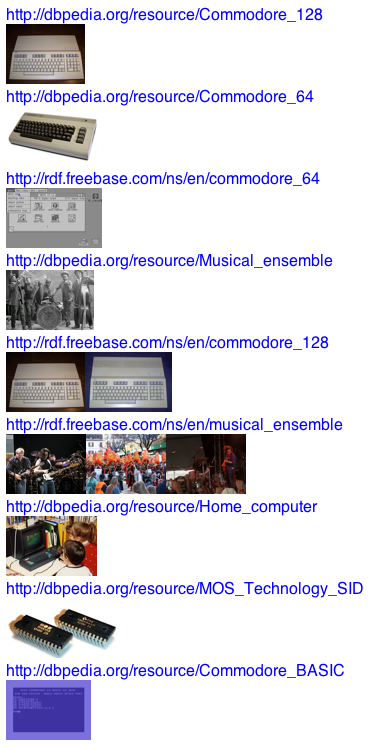
\includegraphics[width=0.44\textwidth]{./resources/semwebvid-entities.png}
    \caption[Depictions for some of the entities from the Commodore 64 music documentary .]{Depictions for some of the entities from the Commodore 64 music documentary available at \url{http://www.youtube.com/watch?v=hzFp3rovfY0}.}   
  \label{fig:c64}
  \end{center}  
\end{figure}

\subsubsection{Media-Content-Ranking}
We have no results yet for this task. We plan to let the user tweak the ranking criteria interactively, and see the effect on the ranking immediately. This could happen via sliders, where a user could change the weights of criteria like view count, duration, recency, etc. The evaluation will happen based on user feedback from a test group. We will have to test whether video genre-specific weights have to be introduced, or whether common weights across all genres reveal satisfactory results.

\subsubsection{Media-Content-Compilation}
We have no results yet for this task. Similar to the previous task \emph{Media-Content-Ranking}, we plan to let the user adjust media composition criteria on-the-fly. For the desired duration, a slider seems adequate, however, we have to do some experiments whether the video compilation can work fast enough to make the slider's reaction seem interactive. The same speed constraint applies to the video composition selection (videos only, images only, combination of both).

Obviously the quality of the final video summaries needs to be evaluated by a test group, ideally against a gold standard of human-generated \emph{event x in n seconds} videos. A typical example is the YouTube \url{http://www.youtube.com/watch?v=skrz1JsxnKc}, which has a 60 seconds summary of Steve Jobs' keynote at WWDC~\cite{wwdc}. The problem, however, with these user-generated summaries is that they usually use official professionally produced video footage, and not user-generated content. This allows for high quality audio and video quality, whereas user-generated content from mobile devices typically suffers from problems like noisy environments when recorded from the middle of an audience, overexposure when recorded against stage lighting, or a lack of detail when recorded from too far away. We will see in how far this is an issue once we have a working prototype of the whole framework.

\section{Future Work}
We split up the description of future work into the different tasks that we have introduced before, and consider general future work separately.
\subsection{Task-related Future Work}
In the following we show task-related future work.

\subsubsection{Event-Selection}
We will keep an eye on a wide variety of events, such as concerts, conferences, political demonstrations, elections, speeches, natural disasters, festivities, but also non-publicly announced events such as private parties, always given there is enough social media coverage and media content available. We will archive social network communication produced around these events for further analysis.

\subsubsection{Micropost-Annotation}
So far we have implemented a solid framework capable of annotating microposts. Future work in this task will be to further increase recall and precision by incorporating more Natural Language Processing engines both for English and non-English languages. While English is covered quite well by the existing engines outlined in Section~\ref{sec:nlp-services}, other target languages such as the so-called FIGS languages (French, Italian, German, Spanish) are still not optimally covered. Our work here will focus on the integration and the alignment of the output formats of the various NLP services, both commercial (such as OpenCalais described in Section~\ref{sec:opencalais}), and non-commercial (such as GATE~\cite{Cun02b}). The main constraint here will be the processing time, and depending on the event the sheer amount of potentially available microposts within a short period of time (compare nation-wide elections with a private party). We will also work on improving entity consolidation and ranking algorithms when different NLP services have agreeing or contradicting results for the same input text.

\subsubsection{Media-Content-Annotation}
At present we have implemented both a command line, and an interactive version of the media content annotation mechanism tailored to the YouTube video platform. Future work in this task will be to improve precision and recall by the same improvement steps as above, similar to the \emph{Micropost-Annotation} task. In addition to these steps, a major improvement will come from piece-wise rather than all-at-once analysis of the available unstructured metadata, taking into account the 300 characters~\cite{andraz} sweet spot mentioned before. The constraint with this task is processing time, especially the more NLP services are involved in processing the data. Our current approach will have to be broadened to support other popular social media video and photo sharing platforms such as TwitVid~\cite{twitvid}, Twitpic~\cite{twitpic}, Lockerz~\cite{lockerz}, yfrog~\cite{yfrog}, Qik~\cite{qik}, Ustream~\cite{ustream}, and Instagram~\cite{instagram}, partly covered by a study on the photo-sharing market shares on Twitter~\cite{techcrunch}. In addition to that we will work to support Facebook's and Twitter's native photo and video sharing offers.

\subsubsection{Media-Content-Ranking}
This task has not started yet. It will consist of development efforts in order to create a testing framework for interactively ranking and re-ranking user-generated media content. A potential paper title for a future publication could be ``Ranking Event-related User-generated Media Content Published Through Social Networks" at conferences or workshops similar to the ACM SIGMM Workshop on Social Media~\cite{wsm2011}.

\subsubsection{Media-Content-Compilation}
This task has not started yet. In a first step, the task consists of application development using JavaScript, HTML5, and CSS in order to generate media content compilations. We will make heavy use of the HTML5 media elements interface~\cite{mediaelements} for the \texttt{video} and \texttt{audio} elements as defined in the HTML5 specification~\cite{w3c_html5}.

In a second step, an evaluation procedure has to be developed in order to objectively judge the generated results. We will investigate in how far existing third party manually generated summaries can be used as a gold standard, or if a self-produced gold standard using only user-generated media content (and not professionally produced content) is necessary.
 
 \subsection{General Future Work} 
We plan on participating in the MediaEval Benchmarking Initiative for Multimedia Evaluation, specifically the Genre Tagging Task~\cite{mediaevalgenre} (2011) and the Social Event Detection Task~\cite{mediaevalevent} (2012). For the prior, we have the infrastructure almost in place with our SemWebVid command line version, described in Section~\ref{sec:semwebvid}. For the latter, we will have substantial content to contribute once our work on the \emph{Media-Content-Ranking} and \emph{Media-Content-Compilation} tasks has matured.

\section{Conclusion}
In this document, we have introduced the overall ideas and visions of the Semantic Web and Linked Data. We have motivated why adding meaning to unstructured information is valuable. In a second step, we have presented Linked Data and Tim Berners-Lee's Linked Data principles and the Linked Open Data cloud. We have examined the state of the art in multimedia semantics and have given an overview of MPEG-7. In continuation we have covered Semantic Web core technologies such as the Resource Description Framework and the Semantic Web query language SPARQL. As an example of Semantic Web technology usage, we have shown Google's Rich Snippets. For the task of structuring unstructured data, we have described Natural Language Processing Web services and URI lookup services that provide links into the Linked Open Data cloud. As a direct application of such structure-giving services, we have demonstrated how communication on social networks can be semantically enriched on-the-fly via Web browser extension mechanisms. We have introduced Media Fragments URIs and their different dimensions for the task of RDF video annotation, which we have described with its sub-tasks entity extraction, URI lookup, and entity depiction. We then have shown how RDF video annotation can work via our interactive Ajax application SemWebVid, or its command line version. Finally we have evaluated our work so far, considering the tasks \emph{Event-Selection}, \emph{Micropost-Annotation}, \emph{Media-Content-Annotation}, \emph{Media-Content-Ranking}, and \emph{Media-Content-Compilation}, and have provided an outlook on future work for each task.

Keeping in mind our objective for this thesis, which is the creation of a framework that allows for the semi-automatic generation of summaries or compilations of several pieces of media content covering a certain event, we feel that we are on the right track. We have the basic bricks in place, both for media content annotation, and for social network communication enrichment. Now we need to put the two pieces together in order to get a working product. We are just getting started\ldots

\pagebreak
\section{Annex A -- Publications}
In the following we list our accepted publications.

\subsection{SemWebVid - Making Video a First Class Semantic Web Citizen and a First Class Web Bourgeois}
Abstract -- SemWebVid is a Web application that allows for the automatic on-the-fly generation of Resource Description Framework (RDF) video descriptions. These descriptions are based on two pillars: first, on a combination of user-generated metadata such as title, summary, and tags; and second, on closed captions which can be user-generated, or be auto-generated via audio transcription services. The plaintext contents of both pillars are analyzed using multiple Natural Language Processing (NLP) Web services in parallel whose results are then merged and where possible detected entities matched back to concepts represented by URIs in the sense of Linked Open Data (LOD). The final result is a downloadable RDF description of the video. As a first exemplary use case the application provides a special view where detected entities are depicted as the video plays along.\\

\noindent For a screenshot of SemWebVid, see Figure~\ref{fig:semwebvid}. A live demo of the application is available at \url{http://tomayac.com/semwebvid/}.\\

\noindent Thomas Steiner. SemWebVid - Making Video A First Class Semantic Web Citizen and A First Class Web Bourgeois. In 9$^{th}$ International Semantic Web Conference (ISWC2010), November 2010.~\cite{semwebvid}

\subsection{SemWebVid - Making Video a First Class Semantic Web Citizen and a First Class Web Bourgeois (Semantic Web Challenge)}
Abstract -- SemWebVid  is an online Ajax application that allows for the automatic generation of Resource Description Framework (RDF) video descriptions. These descriptions are based on two pillars: first, on a combination of user-generated metadata such as title, summary, and tags; and second, on closed captions which can be user-generated, or be auto-generated via speech recognition. The plaintext contents of both pillars are being analyzed using multiple Natural Language Processing (NLP) Web services in parallel whose results are then merged and where possible matched back to concepts in the sense of Linked Open Data (LOD). The final result is a deep-linkable RDF description of the video, and a “scroll-along” view of the video as an example of video visualization formats.\\

\noindent Thomas Steiner and Michael Hausenblas. SemWebVid - Making Video A First Class Semantic Web Citizen and A First Class Web Bourgeois. In Semantic Web Challenge at ISWC2010, November 2010,~\cite{semwebvidswc}.\\

\subsection{How Google is Using Linked Data Today and Vision for Tomorrow}
Abstract -- In this position paper, we first discuss how modern search engines, such as Google, make use of Linked Data spread in Web pages for displaying Rich Snippets. We present an example of the technology and we analyze its current uptake. We then sketch some ideas on how Rich Snippets could be extended in the future, in particular for multimedia documents. We outline bottlenecks in the current Internet architecture that require fixing in order to enable our vision to work at Web scale.\\

\noindent Thomas Steiner, Rapha{\"e}l Troncy and Michael Hausenblas. How Google is using Linked Data Today and Vision For Tomorrow. In Proceedings of Linked Data in the Future Internet at the Future Internet Assembly, Ghent, December 2010, CEUR Workshop Proceedings ISSN 1613-0073, February 2010,~\cite{CEUR-WS.org/Vol-700/Paper5}.\\

\subsection{Fulfilling the Hypermedia Constraint via HTTP OPTIONS, the HTTP Vocabulary in RDF, and Link Headers}
Abstract -- One of the main REST design principles is the focus on media types as the core of contracts on the Web. However, not always is the service designer free to select the most appropriate media type for a task, sometimes a generic media type like application/rdf+xml (or in the worst case a binary format like image/png) with no defined or possible hypermedia controls at all has to be chosen. With this position paper we present a way how the hypermedia constraint of REST can still be fulfilled using a combination of Link headers, the OPTIONS method, and the HTTP Vocabulary in RDF.\\

\noindent Thomas Steiner and Jan Algermissen. Fulfilling the Hypermedia Constraint Via HTTP OPTIONS, the HTTP Vocabulary In RDF, and Link Headers. In Proceedings of the Second International Workshop on RESTful Design, WS-REST ’11, pages 11–14, New York, NY, USA, 2011. ACM,~\cite{Steiner:2011:FHC:1967428.1967433}.\\

\subsection{A Tweet Consumers’ Look at Twitter Trends} 
Abstract -- The Twitter Trends feature allows for a global or local view on ``what’s happening in my world right now” from a tweet producers’ point of view. In this paper, we show the possibility to complete the functionality provided by Twitter Trends via having a closer look at the other side: the tweet consumers’ –- i.e. readers’ -– point of view. While Twitter Trends works by analyzing the frequency of terms and their velocity of appearance in tweets being written, our approach is based on the popularity of extracted named entities (in the sense of Linked Data) in tweets being read. Our experimentation architecture uses a client-side browser extension to harvest and dissect tweets from users’ timelines, search result pages, or profile pages, i.e. tweets supposed to be read. Named entities are extracted via several third-party Natural Language Processing (NLP) Web services in parallel, and are then reported to Google Analytics, which is used to store, analyze, and compute trends by pivoting the reported named entities by Google Analytics data, e.g. users’ geographic locations.\\

\noindent For a screenshot of the Twitter Swarm NLP Chrome extension that was developed in the context of this publication, see Figure~\ref{fig:twitter-swarm-nlp}. The extension is available at \url{http://bit.ly/twitterswarmnlp}.\\

\noindent Winner of the award ``best demo" and ``best poster" at the Making Sense of Microposts workshop (MSM2011).\\

\noindent Thomas Steiner, Arnaud Brousseau, and Rapha{\"e}l Troncy. A Tweet Consumers' Look At Twitter Trends. In Workshop Making Sense of Microposts at ESWC 2011, Heraklion, Crete, May 2011,~\cite{twittertrends}.\\

\subsection{Introducing a Unified Framework for Content Object Description (I-SEARCH)}
Abstract -- In this paper, a novel framework for description of rich media content is introduced. Firstly, the concept of ``Content Objects" is provided. Content Objects are rich media presentations, enclosing different types of media, along with real-world information and user-related information. These highly complex presentations require a suitable description scheme in order to be searched and retrieved by end users. Therefore a novel Rich Unified Content Description is analyzed, which provides a uniform descriptor for all types of Content Objects irrespective of the underlying media and accompanying information.\\

\noindent P. Daras, A. Axenopoulos, V. Darlagiannis, D. Tzovaras, X. Le Bourdon, L. Joyeux, A. Verroust-Blondet, V. Croce, T. Steiner, A. Massari, A. Camurri, S. Morin, A.D. Mezaour, L. Sutton, S. Spiller. Introducing a Unified Framework for Content Object Description. International Journal of Multimedia Intelligence and Security, 2010. Accepted for publication, \url{http://www.inderscience.com/browse/index.php?journalID=359}.

\pagebreak
\section{Annex B -- Demonstrations}
In the following we list our accepted, publicly available, or deployed demonstrations.

\subsection{SemWebVid} \label{sec:semwebvid}
SemWebVid is an Ajax application that allows for the automatic on-the-fly generation of Resource Description Framework (RDF) video descriptions. These descriptions are based on two pillars: first, on a combination of user-generated metadata for a video such as title, summary, and tags; and second, on closed captions, which can be user-generated, or be auto-generated via audio transcription services. This textual information is enriched using multiple Natural Language Processing (NLP) Web services in parallel in order to extract named entities. The resulting named entities are then merged, and wherever possible the detected named entities are matched back to concepts represented by URIs in the sense of Linked Data. The final result is a downloadable RDF description of the video, and a ``scroll-along" view of the video as an example of video visualization formats. At present the application is interactive, i.e. requires user interaction in order to create an RDF video description, however, once the technique has proven to be effective, the process could be automated and become a regular part of video crawling techniques used by general search engines. Figure~\ref{fig:semwebvid} shows a screenshot of the application.

\begin{figure}[htbp!]
\begin{center}
    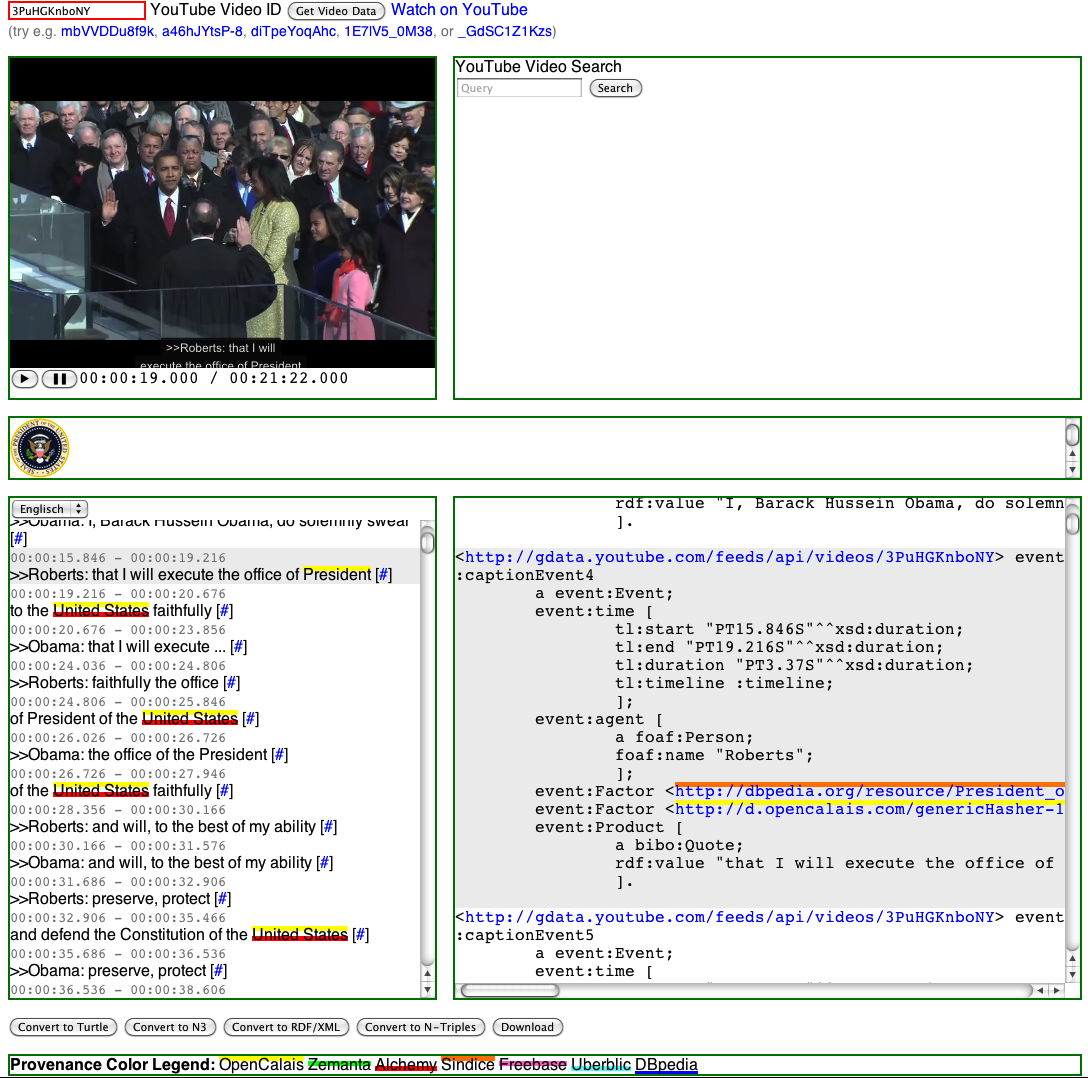
\includegraphics[width=1\textwidth]{./resources/semwebvid.png}
    \caption[Screenshot of the SemWebVid application.]{Screenshot of the SemWebVid application. Demo: \url{http://tomayac.com/semwebvid/}.}    
  \label{fig:semwebvid}
  \end{center}  
\end{figure}

\subsection{Facebook Swarm NLP}\label{fb-swarm}
This extension for the Google Chrome browser performs swarm Natural Language Processing (NLP) on Facebook status updates. The extracted entities are displayed below each status message. In addition to that the extracted entities are then reported to a shared Google Analytics account via the Analytics event tracking code snippet that allows us to create a ranking of the most-talked-about entities. Figure~\ref{fig:facebook-swarm-nlp} shows a screenshot of the extension.

\begin{figure}[htbp!]
\begin{center}
    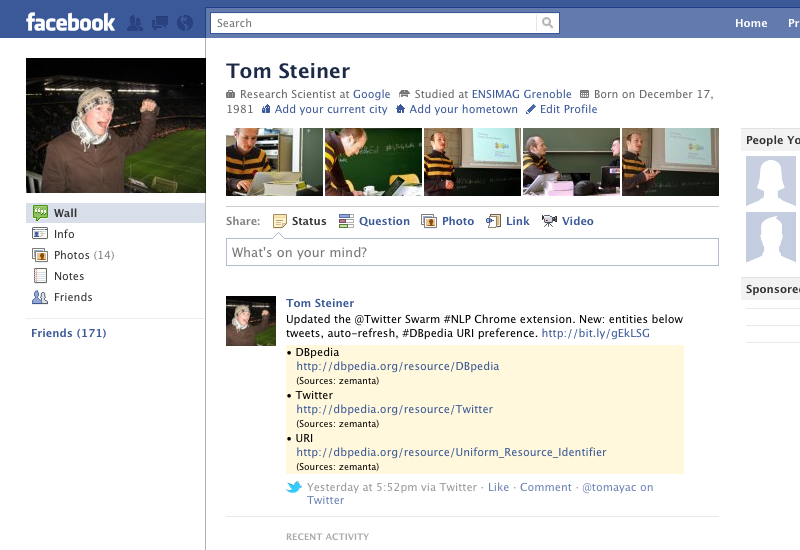
\includegraphics[width=0.7\textwidth]{./resources/facebook-swarm-nlp.png}
    \caption[Facebook Swarm NLP Chrome extension.]{Facebook Swarm NLP Chrome extension. Demo: \url{https://chrome.google.com/webstore/detail/nhcgonkeclhijbkpelhmclmjijphafhk}.} 
  \label{fig:facebook-swarm-nlp}
  \end{center}  
\end{figure}

\subsection{Twitter Swarm NLP}\label{tw-swarm}
This extension for the Google Chrome browser performs swarm Natural Language Processing (NLP) on tweets. The extracted entities are displayed below each tweet. In addition to that the extracted entities are then reported to a shared Google Analytics account via the Analytics event tracking code snippet that allows us to create a ranking of the most-tweeted-about entities. The extension adds an auto-refresh feature to users' timelines that pulls in new tweets automatically when they are available. Figure~\ref{fig:twitter-swarm-nlp} shows a screenshot of the extension.

\begin{figure}[htbp!]
\begin{center}
    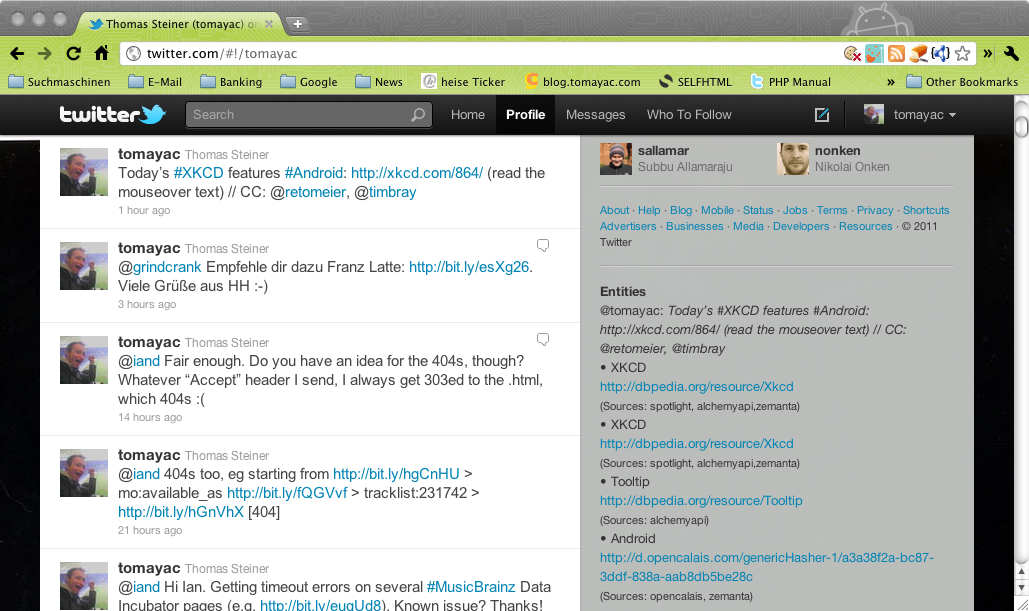
\includegraphics[width=0.7\textwidth]{./resources/twitter-swarm-nlp.png}
    \caption[Twitter Swarm NLP Chrome extension.]{Twitter Swarm NLP Chrome extension. Demo: \url{https://chrome.google.com/webstore/detail/dpbphenfafkflfmdlanimlemacankjol}.}
  \label{fig:twitter-swarm-nlp}
  \end{center}  
\end{figure}

\subsection{GoodRelations Amazon Checker}
This extension for the Google Chrome browser allows for checking whether a \texttt{Product} or \texttt{Offering} as defined by the GoodRelations~\cite{Hepp:GoodRelations} ontology is available on Amazon.com. It is based on the RDFa API~\cite{rdfa:api}, as published by the RDFa Working Group. Figure~\ref{fig:goodrelations-amazon-checker} shows a screenshot of the extension.

\begin{figure}[htbp!]
\begin{center}
    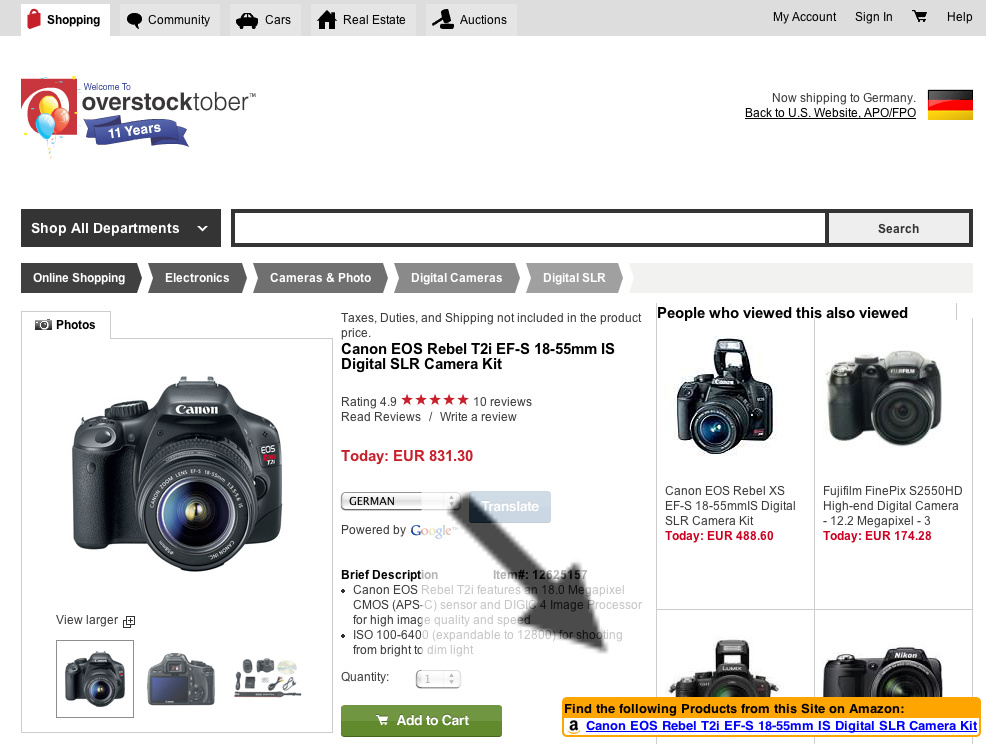
\includegraphics[width=0.7\textwidth]{./resources/goodrelations-amazon-checker.png}
    \caption[GoodRelations Amazon Checker Chrome extension.]{GoodRelations Amazon Checker Chrome extension. Demo: \url{https://chrome.google.com/webstore/detail/jlfealjceojnflopgcelhcmghpakmklk}.}   
  \label{fig:goodrelations-amazon-checker}
  \end{center}  
\end{figure}

\subsection{GoodRelations Currency Converter}
This extension for the Google Chrome browser converts foreign currencies found in GoodRelations~\cite{Hepp:GoodRelations} mark-up on websites to Euro (\euro). It is based on the RDFa API~\cite{rdfa:api}, as published by the RDFa Working Group. Figure~\ref{fig:goodrelations-currency-converter} shows a screenshot of the extension.

\begin{figure}[htbp!]
\begin{center}
    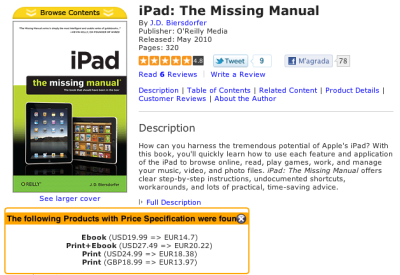
\includegraphics[width=0.7\textwidth]{./resources/goodrelations-currency-converter.png}
    \caption[GoodRelations Currency Converter Chrome extension.]{GoodRelations Currency Converter Chrome extension. Demo: \url{https://chrome.google.com/webstore/detail/nndndkmonaojkllhllgkhfagiakahnki}.}    
  \label{fig:goodrelations-currency-converter}
  \end{center}  
\end{figure}

\subsection{RDFa Triples Lister}
This extension for the Google Chrome browser lists all RDF triples on a website that are embedded in RDFa~\cite{ben_adida_rdfa_2008} format. It is based on the RDFa API~\cite{rdfa:api}, as published by the RDFa Working Group. Figure~\ref{fig:rdfa-triples-lister} shows a screenshot of the extension.

\begin{figure}[htbp!]
\begin{center}
    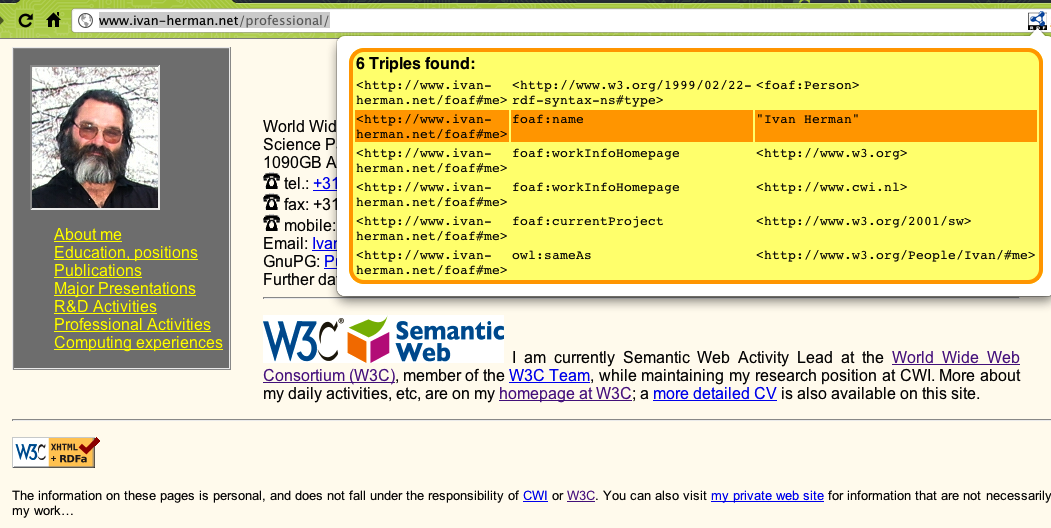
\includegraphics[width=0.7\textwidth]{./resources/rdfa-triples-lister.png}
    \caption[RDFa Triples Lister Chrome extension.]{RDFa Triples Lister Chrome extension. Demo: \url{https://chrome.google.com/webstore/detail/lmojbfnaigeibgkhacnebnpbhddpnoam}.}    
  \label{fig:rdfa-triples-lister}
  \end{center}  
\end{figure}

\subsection{Creative Commons Laser Highlighter}
This extension for the Google Chrome browser highlights any Creative Commons license RDFa~\cite{ben_adida_rdfa_2008} mark-up on websites with a dynamic laser effect. It is based on the RDFa API~\cite{rdfa:api}, as published by the W3C RDFa Working Group. Figure~\ref{fig:creative-commons-laser-highlighter} shows a screenshot of the extension.

\begin{figure}[htbp!]
\begin{center}
    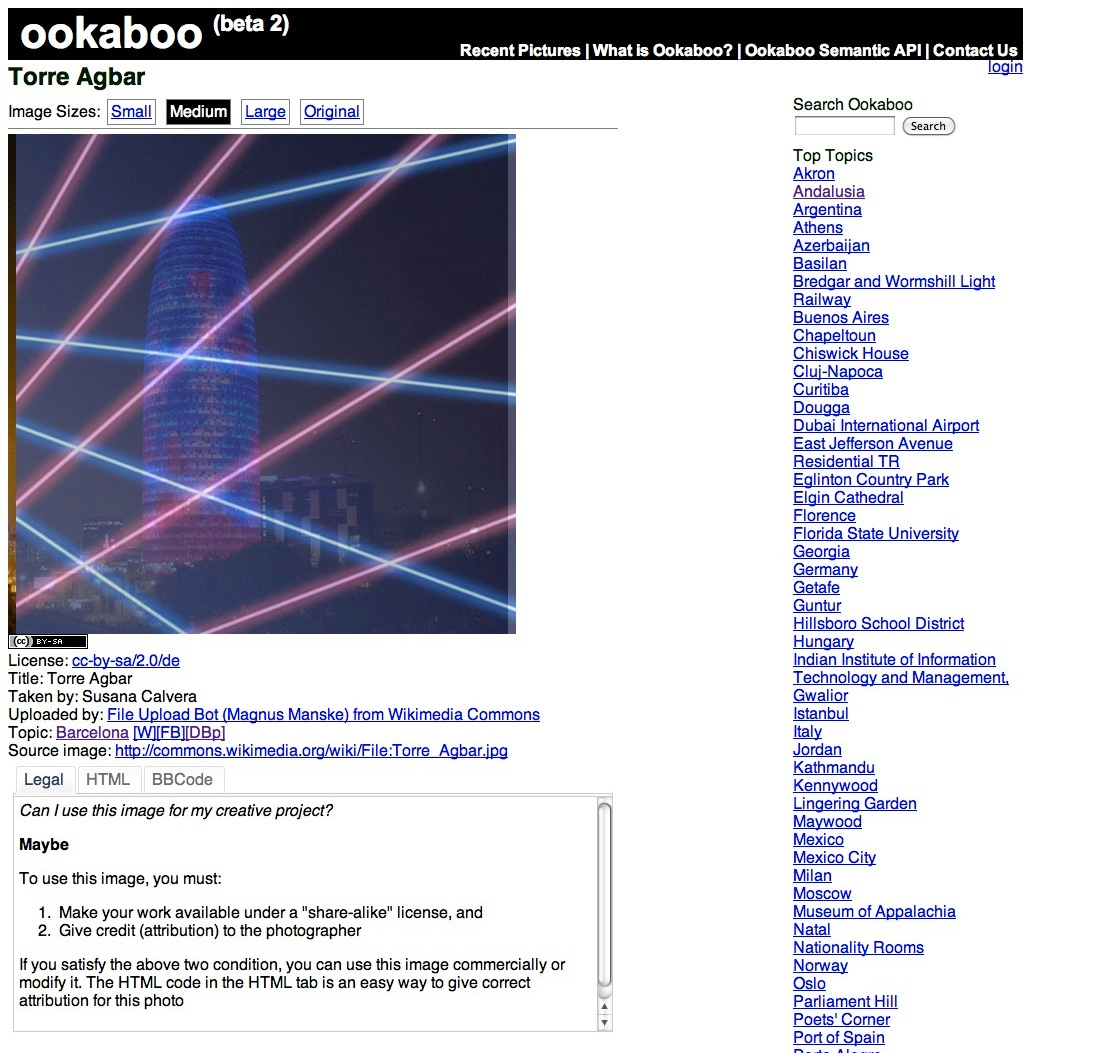
\includegraphics[width=0.7\textwidth]{./resources/creative-commons-laser-highlighter.png}
    \caption[Creative Commons Laser Highlighter Chrome extension.]{Creative Commons Laser Highlighter Chrome extension. Demo: \url{https://chrome.google.com/webstore/detail/iceopjodmdipccjbknbjolkfogkgloei}.}
  \label{fig:creative-commons-laser-highlighter}
  \end{center}  
\end{figure}

\pagebreak
\section{Annex C -- Recommended Literature}
In this Section we present recommended literature for further reading.
\begin{itemize}
\item Mathias Lux, Michael Granitzer, and Marc Spaniol. \emph{Multimedia Semantics -- The Role of Metadata}, Springer, 2008,~\cite{LGSp08}.
\item R. Troncy, B. Huet, and S. Schenk. \emph{Multimedia Semantics: Metadata, Analysis and Interaction}, Wiley-Blackwell, 2011,~\cite{troncy}.
\item Tom Heath, and Christian Bizer. \emph{Linked Data (Synthesis Lectures on the Semantic Web: Theory and Technology)}, Morgan \& Claypool Publishers, 2011,~\cite{heathbizer}.
\item Dean Allemang, and James Hendler. \emph{Semantic Web for the Working Ontologist: Effective Modeling in RDFS and OWL}, Morgan Kaufmann, 2008,~\cite{Allemang}.
\item Toby Segaran, Colin Evans and Jamie Taylor. \emph{Programming the Semantic Web}, O'Reilly Media, 2009,~\cite{Segaran}.
\end{itemize}

\pagebreak
\bibliographystyle{plain}
\bibliography{toc}
\end{document}